%!TEX root = ../2019_7_Ozgumus_Semsi_Yigit.tex
\begingroup
{
	\color{Green}

This chapter is dedicated to the exploration of state of the art approaches in the fields relevant
to the thesis. The organization of the chapter is the following: Section \ref{sec:ad} will formulate
anomaly detection problem and illustrate mainstream approaches towards its solution.  Section \ref{sec:arch_comp} will give
necessary background about generative adversarial networks (GAN) and autoencoder
networks. First, the principles behind how GANs work will be presented then the Autoencoder Networks
 will be explained. This section is particularly significant to understand how different
architectures that use these networks actually work. In Section \ref{sec:gan_based_sota}, variety of 
architectures that has been developed for anomaly detection will be studied as state of the art. 
How they are implemented and their purpose will be described.

\section{Anomaly Detection}
\label{sec:ad}
Anomaly detection can be defined as the task of identifying test data that differs in some respect 
from the data for the model that is available during training \cite{Pimentel:2014:RRN:2588908.2589196}.
This definition correctly describes the task on the abstract level but does not clarify what an anomaly 
actually is. Depending on the the application domain, anomalies can be referred to as outliers, 
novelties, discordant observations, exceptions, aberrations, surprises, peculiarities and
contaminants \cite{Chandola:2009:ADS:1541880.1541882}. Sometimes these terms can be used interchangeably in
the context. These distinctions in the definition primarily rely not only on the features of
the data such as its dimensional complexity, its continuity and format, but also on what is
considered an anomaly for that specific domain. This makes it hard to conceptualize the problem of
anomaly detection with a general definition and a solution that can encompass all different
domains.

In the rest of this section, I will explain different use cases for anomaly detection to show its
impact on a broad spectrum of problems. Then the primary approach types to solve anomaly detection
problem will be introduced.

The categorization taxonomy to define different application domains is constantly changing 
parallel to developments in the literature but the application areas of 
anomaly detection can be categorized down to these five general fields
\cite{Pimentel:2014:RRN:2588908.2589196}.
These are:
\begin{itemize}
    \item IT Sector 
    \item Healthcare informatics, medical diagnostics and monitoring
    \item Industrial Monitoring/ maintanence and damage detection
    \item Image processing/ Video Survailance
    \item Survailance
    \item Sensor Networks
\end{itemize}

\textbf{ IT Sector}

Anomaly detection methods have a huge impact on the IT security systems, in which the objectives
include network intrusion detection and fraud detection \cite{Pimentel:2014:RRN:2588908.2589196}.
With rising use of computerized systems and the incorporation of the internet based services to
our daily lives, maintainability and the availability of these systems became much more important.
For systems like these, anomaly is considered as a priority because it indicates significant but
rare events and can prompt to critical actions to be taken in a domains such as finance or cyber security
\cite{AHMED201619}. For example a malicious process in a server may show increased use of resource
from time to time that may be spotted as a type of anomaly in the system resource use patterns or
the unusual amount of traffic on the network may indicate an intruder attack \cite{FERNANDES20161}
\cite{JABEZ2015338}. Another aspect of the increased use of internet is its impact on the e-commerce
field and dramatically growing online payment systems. This also includes a migration to internet
banking in favor of technological convenience. As a result, insurance and credit card frauds,
scams towards phone and mobile data usage, and phishing attacks targeting financial transactions
become more and more severe \cite{finance_anomaly}. In this context, behavior of the consumer
becomes the data. Transaction history, time spent between consecutive transactions and the
geographic data can be used to construct a model to detect anomalies in the purchase patterns.

\textbf{ Healthcare}

Healthcare and medical diagnostics is another domain for anomaly detection. Detecting anomalies in
the progression of the disease symptoms is a crucial factor for treatment monitoring
\cite{Schlegl2017UnsupervisedAD}. To aid diagnostics, interpretation of the patient data is also an
important task for anomaly detection. Ability to differentiate between the instrumentation or
recording errors and the actual clinically relevant change that may indicate a symptom should also
be present in these anomaly detection systems. \cite{Pimentel:2014:RRN:2588908.2589196}. Patient
data may include tabular information like the age, weight, blood test results, heart or
respiratory rate \cite{inproceedings_medical}\cite{Markou:2003:NDR:959414.959416} or medical image data
\cite{Schlegl2017UnsupervisedAD}. 

\textbf{ Industrial Monitoring}

Novelty detection became a huge part of the industrial automation systems from the quality control
of the manufacturing progress to the performance maintenance of the equipment. Products that have
a complicated and delicate manufacturing process like CPU wafers \cite{Kim:2012:MLN:2076800.2076903} and nanofibrous
materials \cite{Napoletano2018anomaly} may easily develop defects in the manufacturing pipeline. Using
anomaly detection is a viable option to reduce the wasted material and optimize the cost of
producing the target product. Same principle also applies to the equipment used in these pipelines.
Equipment and assets have the risk of deteriorating over time due to the usage
and wear \cite{Pimentel:2014:RRN:2588908.2589196}. For example heavy extraction machines that is used in the
petroleum industry like turbo machines \cite{s150202774} needs constant supervision for damage
prevention. 

\textbf{ Image Processing/ Video Surveillance}

Image processsing methods has been used with anomaly detection methods extensively to detect novelty
subjects or anomalies in the image or in a video stream. Detection in video data stream data is an
important task for the surveilance systems that is used with the purpose of traffic control,
security systems and search and rescue \cite{image_anomaly}.

\textbf{ Sensor Networks}

With the improvements of smart devices' involvement in our daily lives and the recent but promising developments
in the field of internet of things, the definition of acquiring and processing data is evolved.
Various types of sensors, especially wireless, are heavily used to collect huge amount of data to
feed various systems such as surveillance, environmental monitoring, and disaster management
\cite{UlIslam2018}. Anomaly detection methods are important for these systems because the performance and 
maintenance of the these system requires constant monitoring of the acquired data. These distributed 
systems are mainly used to collect and compute the gathered sensory data and predict target information. 
However the accuracy of these computations or predictions depends
primarily on the quality of the sensor measurements and with this scale the instrumentation error
is unavoidable. That's why anomaly detection tasks usually deployed on these systems to observe
sensory faults and also prevent errors caused by malicious attacks \cite{Pimentel:2014:RRN:2588908.2589196} \cite{iot_anomaly}.

Variety of approaches that belong to different sub domains of the machine learning, statistics ,
bayesian and information theory are used to solve anomaly detection problem for these aforementioned
fields. All these different approaches in general tries to build a model or a representation of the
data that is provided which contains no anomalous samples (or very few) and assigns 
them an anomaly score or a label depending on the problem. At the inference stage, deviations from the constructed normality
definition are detected using a predetermined anomaly threshold. These different methods can be
categorized into 5 main titles. These are:

\begin{itemize}
  \item Probabilistic Anomaly Detection Methods
  \item Distance Based Anomaly Detection Methods
  \item Domain Based Anomaly Detection Methods
  \item Information Theoretic Anomaly Detection Methods
  \item Reconstruction Based Anomaly Detection Methods  
\end{itemize}

\textbf{Probabilistic methods} aim to estimate the generative probability density function of the data
with the assumption that the input data is generated from an unknown probability distribution $D$,
and learning this distribution provides us a mathematical representation of normality for the input
data, training set. Anomaly (or novelty in some approaches) score then can be determined which has
certain probabilistic interpretation and can be used to detect the anomaly on the inference stage
\cite{Pimentel:2014:RRN:2588908.2589196}. \textbf{Distance based methods} are another type of 
anomaly detection technique used to model the training data.
Including the K-Nearest neighbour based and clustering based methods, distance based methods rely on
distance metrics between the data points to create a representation for normality. For example
considering the K-NN approach, data points in the training dataset are identified to have close
neighbour points using the distance metrics while a sample that has greater distance to the
nearest normal point is identified as an anomaly. \textbf{Domain based methods} creates a 
boundry based on the structure of the training dataset \cite{Pimentel:2014:RRN:2588908.2589196}.
These methods are usually insensitive to
different sampling or the density properties because instead of learning the density of
the data, the learn the boundary information to seperate the target class (anomalies) from the
normal data. Support Vector Machines (SVM) are the popular example for this approach. \textbf{Information
theoretic anomaly detection methods} computes the total information content that resides in the
training dataset. The main assumption is that anomalous samples present in the data significantly
modifies the information content of the assumed normal dataset. Metrics for this approach are
calculated using the entirety of the dataset and the subset that triggers the biggest discrapancy is
identified as the anomaly. 

\textbf{Reconstruction based methods} which also is the focus of this thesis, model the underlying
representation of the data and reconstructs it. Using the original input and the reconstructed
output, these models define a reconstruction error tailored to the nature of the problem and the
type of data, and measures this error with respect to certain anomaly threshold. Since the modeled
underlying data has the features specific to the training dataset, when the anomalous sample is
fed through this pipeline, its representation and consequently its reconstruction will be made
poorly hence giving a greater reconstruction error. 

\subsection{Related Works}
\label{sec:relworks}

In this subsection, previous works and state of the art related to anomaly detection in images 
and proceed with particular case of SEM images (see section \ref{sec:sem}) are presented. Proposed 
methods for anomaly detection for images can be grouped in reference-based and reference-free ones 
\cite{Chandola:2009:ADS:1541880.1541882}. Reference-based approaches compares the input image with a 
template image which is anomaly-free by definition and result of this comparison decides in run-time 
whether input includes anomalous component or not \cite{zontak2010defect}.
However, they are not feasible for considered SEM images where filament structures follow
randomized rather than geometric pattern \cite{carrera2016defect}. Considering this distinction, our proposed model 
is a member of reference-free approach which learns to model the data with an unsupervised setting.

This problem of particular dataset of SEM images previously studied in \cite{carrera2016defect},
\cite{carrera-2016-scale} and \cite{boracchi2014novelty} and these methods are based on learning a 
sparse dictionary that represents the normal regions and in run-time, if the input does not conform 
with the learned dictionary, it is detected as anomalous. Another approach that introduces convolutional 
neural networks to anomaly detection task in SEM images is established by Napoletano et al. \cite{Napoletano2018anomaly}. 
To extract feature for "normality" concept, they exploit pretrained network called ResNet \cite{he2016deep} 
which consists of residual networks and trained by large number of images. After feature extraction, 
for test phase, they create a dictionary by using K-means clustering from normal subregions in the training data 
and use this to compare with test samples to determine the degree of abnormality \cite{Napoletano2018anomaly}.

Another powerful model for novelty detection is autoencoders (see Section \ref{sec:ae}). Autoencoders are quite useful 
tools to learn the dynamics of a distribution defined over images and to generate examples that corresponds 
to a sample on learned distribution. Therefore, they are easily deployed for novelty 
detection as in \cite{an2015variational}, \cite{leveau2017adversarial} and
\cite{Pidhorskyi:2018:GPN:3327757.3327787}. Particularly, in Sabokrou et al.\cite{sabokrou2018adversarially},
leverages two staged network that is composed by auto-encoders and convolutional neural networks is explored for
the novelty detection. 

Next section will introduce generative adversarial networks and autoencoder networks to give background for the 
GAN based anomaly detection frameworks introduced in Section \ref{sec:gan_based_sota}. In Section \ref{sec:gan}, Underlying mechanics of 
adversarial training and how generative adversarial networks learn to generate given data will be explained. Regarding 
autoencoder networks, main principle behind their implementation and how they are trained to obtain a latent representation of a given 
data will be described.


\section{Architectural Components}
\label{sec:arch_comp}
This section introduces the two main network types used in  anomaly detection
frameworks. Section \ref{sec:gan} will describe how generative adversarial network
framework is formed and the intuition behind its adversarial training scheme. Section 
\ref{sec:ae} will give an introductory information to autoencoder networks and present different kinds of
approaches that can be integrated into both the construction of the network and its training
methodology. 

\subsection{Generative Adversarial Networks}
\label{sec:gan}

One of the main objectives of the deep learning is to create complex and high dimensional
models that can capture the relations amongst the fundamental types of data that we work with. 
This data may differ, it can be a visual information like an image,
symbols in natural language or audio waveforms containing speech. We then use these models to make
machines make sense of the world we live in and exhibit what we call an intelligence
\cite{Bengio:2009:LDA:1658423.1658424}.

In the terms of statistical classification, also in machine learning, two main approaches for building 
classifiers are called discriminative and generative modelling. They differ in the degree of statistical 
modelling\cite{gdjabra}. Discriminative models maps the rich, complex sensory data to a class label to
perform the desired task. They try to learn the conditional probability distribution of the input
data using the features of the data. Success behind this approach is the result of the
improvements in the training, learning and generalization of these models. Back propagation
\cite{Widrow2008AppendixGT}, dropout \cite{Srivastava2014DropoutAS}, and rectified linear
units\cite{Glorot2011DeepSR} are some of the example concepts that contribute to this success.

Generative models try to estimate the joint probability distribution of the high dimensional sensory 
input data to be able to generate data similar to input and its label with some variations which can be 
thought as imaginative. Latest models such as Boltzmann machines \cite{Salakhutdinov2009DeepBM} and Gaussian Mixture Models 
\cite{Reynolds2009GaussianMM} did not show a considerable promise as opposed to discriminative models mainly 
because of the type of problem they try to solve and computational difficulties regards to its solution. 
It is observed that main difficulty was the probabilistic computations that are hard to control in the maximum 
likelihood estimation \cite{Goodfellow:2014:GAN:2969033.2969125,pmlr-v5-salakhutdinov09a}.

Generative Adversarial Networks (GAN)\cite{Goodfellow:2014:GAN:2969033.2969125} are considered as one of 
the most significant breakthroughs in deep learning and generative modelling in the recent years. Framework 
consists of a generator and discriminator network. You can observe the example architecture in the Figure 
\ref{fig:gan_network}. 

\begin{figure}[h]
	\centering
	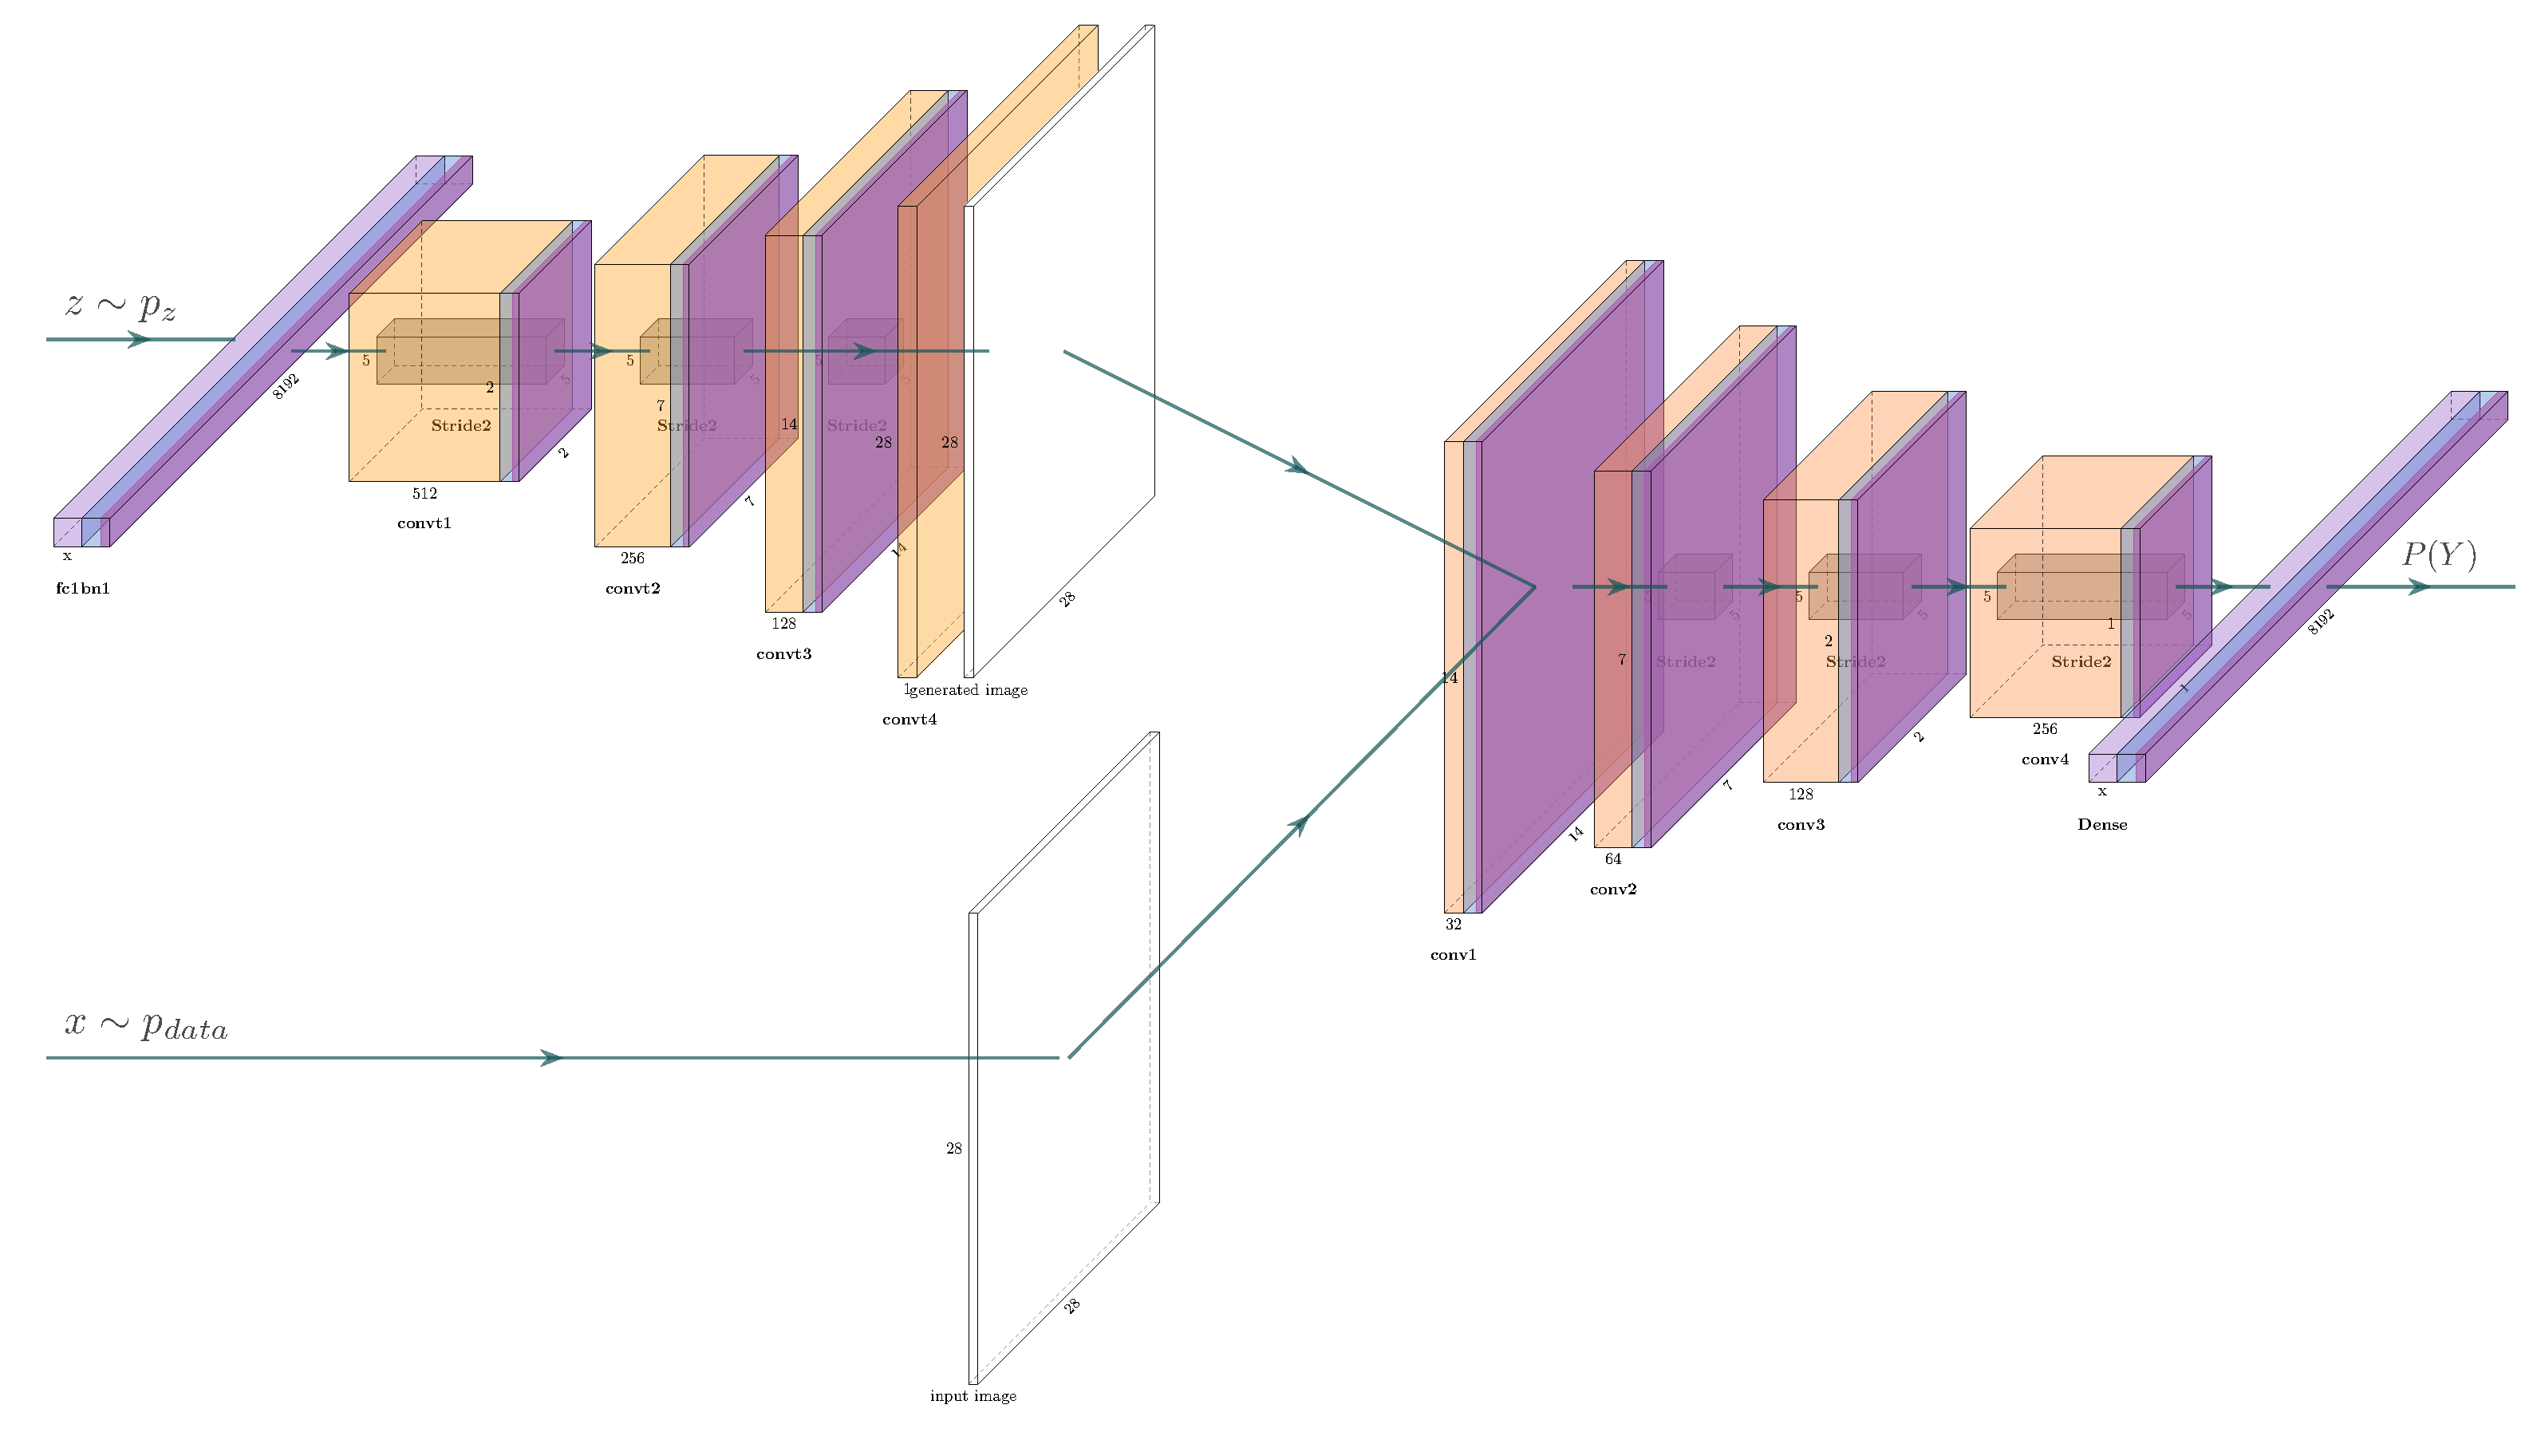
\includegraphics[width=.9\textwidth]{gan}
    \caption{GAN architecture overview}
    \label{fig:gan_network}
\end{figure}

From this point on, "image" will be used to specify the type of the input and the target data because
GAN frameworks are mainly designed to work with high dimensional spatial data like images so it will
be consistent when explaining the theorem and also the central focus of the thesis is on the spatial
data. 

Power of this framework comes from the adversarial nature of the training process. Simply put,
the goal of generator network($G$) is to create images similar to the input data by capturing the
data distribution using a probabilistic model. On the other hand discriminator ($D$) tries to detect fake
(generated) images that is created by generator from the real input images. We can represent this intuition 
with the following two player mini-max game with the value function $V(G,D)$ in Equation \ref{eqn:gan_vgd}. 
Here $P_{\text{data}}$ represents the probability distribution of the data that we have no information about. 
$p_z(z)$ is the random noise that generator accepts to generate fake data 
\cite{Goodfellow:2014:GAN:2969033.2969125}.
\begin{align}
    p_{\text{data}} (x) & : x \in \Omega_{X} \quad (\text{Distribution of the data})\\[5pt]
    p_z (z) & : z \in \Omega_{Z} \quad (\text{Distribution of the noise}) \\[5pt]
    \label{eqn:gan_vgd}
    V(G, D) &= \mathbb{E}_{\boldsymbol{x} \sim p_{\text { data }}(\boldsymbol{x})}[\log D(\boldsymbol{x})]+\mathbb{E}_{\boldsymbol{z} \sim p_{\boldsymbol{z}}(\boldsymbol{z})}[\log (1-D(G(\boldsymbol{z})))]
\end{align}

Training objective for the discriminator is to maximize the expected log-likelihood of
classifying the input data as real.
Since generated data should be classified as fake by the discriminator, output of the second
term is flipped. The Generator's purpose is to "fool the discriminator". Hence its objective
is to minimize the expected log likelihood of discriminator classifying generated image sample as
fake. We can interpret this equation as two separate objective functions with different training
criteria :
\begin{align}
    \min _{G} V(G, D)=& \mathbb{E}_{\boldsymbol{z} \sim p_{\boldsymbol{z}}(\boldsymbol{z})}[\log (1-D(G(\boldsymbol{z})))] \\[5pt]
    \max _{D} V(G, D)=& \mathbb{E}_{\boldsymbol{x} \sim p_{\text { data }}(\boldsymbol{x})}[\log D(\boldsymbol{x})]+\mathbb{E}_{\boldsymbol{z} \sim p_{\boldsymbol{z}}(\boldsymbol{z})}[\log (1-D(G(\boldsymbol{z})))]
\end{align}

While this equation describes the relation between two adversaries, it does not provide a
definite explanation how this training objective finds equilibrium and whether that equilibrium also
provides us with the optimal generator or not. For this analysis we will use bottom up approach and
prove the theorem depicted in the original GAN method \cite{Goodfellow:2014:GAN:2969033.2969125}. Here,
$C$ is defined as the function of training criterion for discriminator $D$ that accepts any generator $G$.

\begin{theorem}
\label{thr:gan}
The global minimum of the virtual training criterion $C(G)$ is achieved if and only if $p_g = p_{\text{data}}$.
At that point, $C(G)$ achieves the value $-log(4)$.
\end{theorem} 
We start by defining the term expected value of a function. 

\begin{definition}
    $E(f(x))$ of some function $f(x)$ with respect to  certain probability distribution
$p(x)$ is called the expected value of a function.  
\end{definition}

It is expressed as:
\begin{equation}
    \label{eqn:ev}
    E_{x \sim p_x} = \int p(x) f(x) dx
\end{equation}

So the minimax game equation can be transformed into Equation \ref{eqn:minmax_gan} : 
\begin{equation}
    \label{eqn:minmax_gan}
    V( G, D) = \int_x p_{\text{data}}(\boldsymbol{x}) log(D(\boldsymbol{x})) dx + \int_z p_z(\boldsymbol{z}) log(1 - D(G(\boldsymbol{z}))) dz
\end{equation}

For generator to sample an image good enough to fool the discriminator, framework needs to learn the
implicitly created sample distribution $p_g$ by the generator $G$. Framework defines a prior noise
distribution $z \sim p_z$, isotropic Gaussian distribution with zero mean and unit variance to learn
the distribution $p_g$ (Different distributions are also considered). Conceptually $p_z$ represents the 
latent features of the data artificially created. While training GAN, semantic meaning of this noise is not controlled.
Next we use the LOTUS theorem.

\begin{theorem}
Law of the unconscious statistician (LOTUS) theorem is used to compute the expected value of a 
function $g(x)$ of a random variable $X$  when one knows the probability distribution of $X$ but 
does not know the probability distribution of $g(x)$ \text{\cite{ringner2009law}}.
\end{theorem}

The expected value of a function $g(x)$ then can be expressed like:
\begin{equation}
    \mathrm{E}[g(X)]=\sum_{x} g(x) f_{X}(x)  
\end{equation}

$f_{X}(x)$ being the probability distribution of the random variable $X$. 

Using this law we can write the equation for $V(G, D)$. 
\begin{align}
    z \sim p_z , \quad G(z) &= x, \quad x \sim p_g\\ 
    V( G, D) &= \int_x p_{\text{data}}(\boldsymbol{x}) log(D(\boldsymbol{x})) + p_g(\boldsymbol{x}) log(1 - D(\boldsymbol{x})) dx
\end{align}

For the Discriminator $D$, the value of the training criterion should be maximized. That basically means the
function derivative of this expected value expression should be equal to zero. We write the
function by reversing the process of Equation \ref{eqn:ev}.
\begin{align}
    f( p_{\text{data}}, p_g) &= p_{\text{data}}(\boldsymbol{x}) \log(D(\boldsymbol{x})) + p_g(\boldsymbol{x}) \log(1 - D(\boldsymbol{x})) \\[5pt]
    f^{\prime} &= p_{\text{data}}(\boldsymbol{x}) \frac{1}{D(\boldsymbol{x}) \ln(C)} - p_g(\boldsymbol{x}) \frac{1}{(1- D(\boldsymbol{x})) \ln(C)} \\[5pt]
    f^{\prime} &= 0
\end{align}
\begin{align}
    p_{\text{data}}(\boldsymbol{x}) (1- D(\boldsymbol{x})) \ln(C) &= p_g(\boldsymbol{x}) D(\boldsymbol{x}) \ln(C)\\[5pt]
    (p_{\text{data}}(\boldsymbol{x}) +  p_g(\boldsymbol{x})) D(\boldsymbol{x}) &= p_{\text{data}}(\boldsymbol{x})\\[5pt]
    D^{*}_G(\boldsymbol{x}) &= \frac{p_{\text{data}}(\boldsymbol{x})}{(p_{\text{data}}(\boldsymbol{x}) +  p_g(\boldsymbol{x}))}\label{eqn:opt_d}
\end{align}

This is the optimal discriminator $D$ with fixed $G$. By deriving this value, we show that the
maximum value Discriminator $D$ can reach is the result of Equation \ref{eqn:opt_d}. Next, we reformulate our
$V(G, D)$ to analyze for the training criterion of the generator $G$. 

\begin{align}
    C(G) &= \max _{D} V(G, D) \\[5pt]
    & =\mathbb{E}_{\boldsymbol{x} \sim p_{\mathrm{data}}}\left[\log D_{G}^{*}(\boldsymbol{x})\right]+\mathbb{E}_{\boldsymbol{z} \sim p_{\boldsymbol{z}}}\left[\log \left(1-D_{G}^{*}(G(\boldsymbol{z}))\right)\right] \\[5pt]
    & =\mathbb{E}_{\boldsymbol{x} \sim p_{\mathrm{data}}}\left[\log D_{G}^{*}(\boldsymbol{x})\right]+\mathbb{E}_{\boldsymbol{x} \sim p_{g}}\left[\log \left(1-D_{G}^{*}(\boldsymbol{x})\right)\right] \\[5pt]
    & =\mathbb{E}_{\boldsymbol{x} \sim p_{\mathrm{data}}}\left[\log \frac{p_{\mathrm{data}}(\boldsymbol{x})}{P_{\mathrm{data}}(\boldsymbol{x})+p_{g}(\boldsymbol{x})}\right]+\mathbb{E}_{\boldsymbol{x} \sim p_{g}}\left[\log \frac{p_{g}(\boldsymbol{x})}{p_{\mathrm{data}}(\boldsymbol{x})+p_{g}(\boldsymbol{x})}\right] 
\end{align}

In the theorem, equality $ p_{\text{data}} = p_g$ is given. By applying this equality we get
$D^{*}_G(\boldsymbol{x}) = \frac{1}{2}$. By putting this to our equation we get:
 $$C(G) = \log(\frac{1}{2}) + \log(\frac{1}{2}) = - \log(4)$$
To verify that this value is indeed the global
point for the equation we apply the following subtraction: 
\begin{multline}
    \label{eqn:gan_optim_proof}
    \begin{split}
        C(G)-(-\log (4))  =\int p_{\text {data}}\left[\log \frac{p_{\text {data}}}{p_{\text {data}}+p_{g}}+\log 2\right]+\\ \int p_{g}\left[\log \frac{p_{g}}{p_{\text {data}}+p_{g}}+\log 2\right]
    \end{split}\\[5pt]
    C(G)-(-\log (4)) =\int p_{\text {data}}\left[\log \frac{2 p_{\text {data}}}{p_{\text {data}}+p_{g}}\right]+\int p_{g}\left[\log \frac{2 p_{g}}{p_{\text {data}}+p_{g}}\right]\\[5pt]
    C(G)-(-\log (4)) =\int p_{\text {data}}\left[\log \frac{p_{\text {data}}}{\left(p_{\text {data}}+p_{g}\right) / 2}\right]+\int p_{g}\left[\log \frac{p_{g}}{\left(p_{\text {data}}+p_{g}\right) / 2}\right]
\end{multline}

To interpret this result we introduce 2 divergence definitions.
\begin{definition}
    The Kullback-Leibler divergence is the measure of how one probability distribution is different from
    the other one.   
\end{definition}
Its general definition is:
\begin{equation}
    D_{K L}(P \| Q)=\int p(x) \log \frac{p(x)}{q(x)}
\end{equation}

More generally if $P$ and $Q$ are probability measures\footnotemark  over a dataset $X$, and measure
$P$ is absolutely continuous with respect the $Q$, then the Kullback-Leibler divergence can also be
defined as in Equation \ref{eqn:kl}

\footnotetext{A probability measure is a real-valued function defined on a set of events in a probability 
	space that satisfies measure properties such as \textit{countable additivity}\cite{Roussas:1614120}}
\begin{equation}
    \label{eqn:kl}
    D_{\mathrm{KL}}(P \| Q)=\int_{\mathcal{X}} \log \left(\frac{d P}{d Q}\right) d P
\end{equation}

where $(f_{PQ}) \coloneqq \frac{d P}{dQ} $ is the Radon-Nikodym derivative \cite{Bill86}. The defining property of
Radon-Nikodym property that ties to the probability measure is that:
\begin{equation}
    \label{eqn:radon}
    P(R) = \int_{R} f_{PQ} d Q
\end{equation}

The RN derivative $f_{PQ} : \Omega \mapsto \mathcal{R}_{\geq 0}$ is defined for any measures $P$ and
$Q$ on a space $\Omega$ such that $P$ is absolutely continuous with respect to $Q$. In other words,
for any $ R \subseteq  \Omega : P(R) > 0 \implies Q(R) > 0$  \cite{Bill86}.

Jensen-Shannon divergence is another measure of similarity between different probability
distributions.  Its major difference from the KL divergence is that it is always symmetric and it
always has a non-negative value. The General definition is provided in Equation \ref{eqn:jsd}.
\begin{equation}
    \label{eqn:jsd}
    J S D(P \| Q)=\frac{1}{2} D_{K L}(P \| M)+\frac{1}{2} D_{K L}(Q \| M)
\end{equation}

Using this divergence measures we can rewrite our equation as this:
\begin{align}
    \label{eqn:gan_eqaul}
    C(G)&=-\log (4)+K L\left(p_{\text { data }} \| \frac{p_{\text { data }}+p_{g}}{2}\right)+K L\left(p_{g} \| \frac{p_{\text { data }}+p_{g}}{2}\right) \\
    C(G)&=-\log (4)+2 \cdot J S D\left(p_{\text { data }} \| p_{g}\right)
\end{align}

Considering Jensen-Shannon divergence is always non-negative and zero only when the distributions
are identical, we can conclude the proof by stating that the global minimum point of $C^*(G) = -
\log(4)$ is only achieved when $p_{\text{data}} = p_g$ .

Intuition behind the adversarial training of this framework is important because all the subsequent
approaches that will be discussed in the thesis that use GAN's fundamentally benefit from this
framework to train their networks. As we will see in the BiGAN (Section \ref{sec:bigan}) and subsequent models, addition of
encoder network changes the overall minimax game played by the adversarial networks but underlying
logic still depends on the value function of the GANs.

\subsection{Autoencoder Networks}
\label{sec:ae}
 
Autoencoder network is a type of neural network that is trained to copy its input data to output
\cite{Goodfellow-et-al-2016}. In its simplest form, it can be defined as a feedforward, 
non-recurrent network similar to multilayer perceptrons like in Figure \ref{fig:ae_simple}.
\begin{figure}[h!]
	\centering
	\includegraphics[width=.75\textwidth]{ae_simple}
    \caption{Simple Autoencoder architecture}
    \label{fig:ae_simple}
\end{figure}

Internally, it consists of a hidden layer that describes the code (latent representation) 
learned from the input data. Connections from the hidden layer to the output layer transforms 
the latent representation into the output data with the same dimensional complexity as the input 
data. It is the composition of two operations. Mapping from input to hidden layer is called encoding. 
Reconstructing data from the code using the mapping from hidden layer to output layer is called 
decoding. However rather than trying to reconstruct the given data, autoencoders are mainly used 
to learn the representation about the data to extract meaningful features and to reduce the 
dimensionality of data while keeping the relevant information.

\begin{figure}[h!]
	\centering
	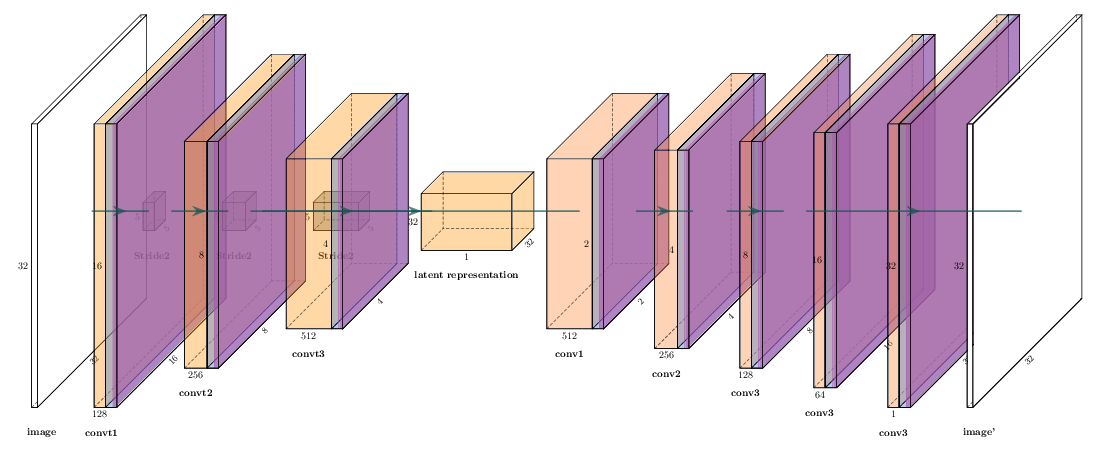
\includegraphics[width=.9\textwidth]{autoencoder}
    \caption{Stacked Autoencoder with multiple layers}
    \label{fig:ae_deep}
\end{figure}

This architecture can be extended to capture more
complex feature representations by stacking similar but varying encoder and decoder layers on top of
each other. With increasing number of layers encoding and decoding operations can be considered as two separate 
networks that is connected by the latent representation connection. Generally first layers learn the more basic features 
of the data and as the layers are stacked, more concentrated and complex features can be learned in the code section 
of the autoencoder, end of the encoder network. These architectures are mainly referred to as deep
autoencoders because of the increased level of hidden layers present in the model depicted in Figure
\ref{fig:ae_deep}.

Learning rationale of the autoencoders can be visualized with a pair of weighted layer computation
functions like in the multilayer perceptrons. Assume that we have two transition functions that
defines the relationship between the real data $X$ and the latent representation $F$ as the result of
the encoder and decoder networks:
\begin{align*}
    \phi : X \mapsto F \\
    \psi : F \mapsto X     
\end{align*}

We can define the intermediate representation computation and the reconstruction of input data
with the following equations:
\begin{align}  
    z  &= \sigma( W x + b) ,\quad x \sim X \in \mathbb{R}^d ,\quad z \sim F \in \mathbb{R}^p \\
    x'  &= \sigma' (W' z + b') 
\end{align}

Training objective for the autoencoders based on reconstruction loss. Depending on the
architecture of the decoder or the desired task, the source of parameters for the objective
function can change. Autoencoder learns the representation of data by minimizing the objective function 
defined as the reconstruction loss. 
\begin{align}
    \label{eqn:ae_rec}
  \phi, \psi & = \underset{\phi, \psi}{\text{argmin}} \norm{X - (\psi \circ \phi) X} \\  
  L(x, x') & = \norm{x - x'}^2 = \norm{x - \sigma' (W' \sigma (W x + b) + b')}^2
\end{align}

With enough model capacity and training time, autoencoder may learn to copy the input perfectly.
This reduces the functionality of encoder-decoder networks to a identity function:
$$
 x \sim X \in \mathbb{R}^d, \quad \psi(\phi(x)) = x
$$

This is generally an unwanted outcome. To overcome this problem, autoencoders are designed to learn the
representation of data imperfectly \cite{Goodfellow-et-al-2016}. This is achieved by how the
encoder network learns to compress the data to a meaningful representation. These 3 types of
autoencoder models can give an idea about how the architecture can be changed to alter the amount of
information that can be extracted from the data. These are:

\begin{itemize}
    \item Undercomplete Autoencoders
    \item Regularized Autoencoders
    \item Denoising Autoencoders
    %\item Variational Autoencoders
\end{itemize}

\textbf{Undercomplete autoencoders} reduce the dimension size of the latent representation. Learning
purposefully insufficient representation forces autoencoder to keep the most salient features about
the data. Training objective function is the reconstruction loss which presented in Equation
\ref{eqn:ae_rec}. If the computation of this function is linear, then the autoencoder mimics the
behaviour of a linear dimensionality reduction methods. When the encoder transition $\phi$ and the
decoder transition $\psi$ is designed to have a nonlinear nature, then the autoencoder has the
ability to capture more complex reprensetation of the data, more powerful approach than known dimensionality 
reduction methods such as Principal Component Analysis. But this has the risk of again, causing 
autoencoder to replicate the input data perfectly and becoming an identity function $x' = \psi(\phi(x))$. 
 Design difference of \textbf{regularized autoencoders} is that their latent representation layer usually has same 
or higher dimensional power (more neurons from the perspective of multilayer perceptrons). 
To acquire a similar performance like undercomplete variants, they regularize the loss function  
with the potential properties of the data distribution such as robustness to the noise or the 
sparsity of the representation. Prioritizing which aspects of the data will be used as a regularizer 
term for the objective function is a task dependent problem \cite{Goodfellow-et-al-2016}. 
\textbf{Denoising autoencoders} tries to solve a different problem to achieve a good representation. 
$$
\hat{x} = x + \epsilon : x \sim X \in \mathbb{R}^d ,\quad \epsilon \sim \mathcal{N}(\mu, \sigma^2)
$$

The input data is corrupted with a Gaussian noise. Denoising autoencoders tries to
reconstruct the data and undo this corruption by minimizing this updated loss with the difference of
$\hat{x}$.
$$
L(x, \psi(\phi(\hat{x})))
$$
Adding noise to the input data forces autoencoder to learn more salient features of the input data and because 
the input is constantly noisy, autoencoder gains a factor of robustness.

In the remaining part of this thesis, generative adversarial networks and autoencoder networks will be referenced 
several times. They constitute the building blocks of all the models presented in the next section. Our proposed 
model's architecture also structured using these networks so their underlying logic is fundamental to understand 
to compose our solution.

\section{GAN Based Anomaly Detection Methods}
\label{sec:gan_based_sota}
In the field of reconstruction based anomaly detection, autoencoder networks 
are fairly popular with spatial data \cite{baldi2012autoencoders,leveau2017adversarial,an2015variational}.
GAN based approaches in this field are relatively new compared to their other variants.
In the following subsections, we will explain the approaches that can be considered as the state of
the art for this problem in the order of their complexity and incremental improvements. Each
model will be evaluated by their problem description, the type of data they use, model
architecture and anomaly score computation. 

\subsection{AnoGAN}
\label{sec:anogan}
 AnoGAN is the first model that utilizes GANs for the anomaly detection task in our knowledge
\cite{Schlegl2017UnsupervisedAD}. It focuses on the problem of detecting anomalous regions in optical
coherence tomography images. Images containing retinal fluid or hyperreflective foci (indicator of
disease progression in various retinal diseases) are identified as anomalous examples. Main
motivation to use GANs to obtain a model which represents normal anatomical variability of the data
is that previous supervised approaches involves training a model with a large dataset using
annotated examples of known markers. Relying on vocabulary of markers may limit the predictive power
of the model as the image contains much more relevant information than the marker and extensive
supervised training is a problem because it means that every stage of the disease requires an
extensive training with annotated examples such as labeled lesions which may decrease limit of
exploiting imaging data for treatment decisions \cite{Schlegl2017UnsupervisedAD}.


The framework consists of 2 parts. First part is the GAN module, generator and discriminator
networks (see Figure \ref{fig:gan_network}). Their architecture is inspired by the original DCGAN
\cite{Radford2016UnsupervisedRL} which contains convolutional layers instead of multi layer perceptron 
layers. The objective function of the GAN is the same of the Equation \ref{eqn:gan_vgd}. 
During the training generator enhances its ability to generate more realistic
retinal images while the discriminator learns to diagnose the real and the generated samples more
efficiently. 

The second part of the framework is about the inverse mapping from the latent space to the image space. 
We know from the GANs training procedure that when the adversarial training is completed, the generator
network has learned the distribution $p_g$ that is theoretically very similar to the input data
distribution $p_{\text{data}}$. ( we state "theoretically" explicitly because depending on the
configuration of GAN and the data that is used, this may differ significantly in practice.) 
Even though with the trained generator $G$, 
$$
G(z) = z \mapsto x,x \sim p_{\text{data}}
$$

the GAN framework does not learn the inverse mapping from the image to noise. AnoGAN framework
aims to find the noise sample $z\prime$ from the query image (normal or anomalous) such that the
generated image $G(z\prime)$ is visually the most similar one to the query image. This is essential
for the anomaly detection task. $z\prime$ is sampled randomly as initialization. Then the
$G(z\prime)$ is computed and based on the defined loss function gradients the coefficients of
$z\prime$ is updated using back propagation. This procedure is repeated for a number of epochs to
obtain the final value of the $z\prime$. 

The loss function for the inverse mapping is defined as the combination of two separate losses.
\textbf{Residual loss} $L_R$ is responsible for enforcing visual similarity between the generated image
$G(z\prime)$ and the query image $x$.
\begin{equation}
    \label{eqn:anogan_rl}
    L_R (z_{\gamma}) = \sum \norm{ x - G(z_{\gamma})}
\end{equation} 
\textbf{Discrimination loss} $L_D$ on the other hand enforces the
generated image $G(z\prime)$ to lie on the manifold $X$ of image $x$.
\begin{equation}
    \label{eqn:anogan_dl}
    L_D (z_{\gamma}) = \sum  \norm{f(x) - f(G(z_{\gamma})}
\end{equation}

There are two different implementation for the discrimination loss. One with sigmoid cross entropy
which is from the original GAN implementation \cite{Goodfellow:2014:GAN:2969033.2969125} and one
with feature matching \cite{fm} which uses the last layer of the discriminator rather than the
output to compute the loss. Using this loss allows them to use discriminator not as a classifier but
as a feature extractor. Using both residual and discrimination loss, the total loss function is
defined as :
$$L(z_{\gamma}) = (1 - \lambda ) \times L_{R}(\boldsymbol{z_{\theta}}) + \lambda \times
L_{D}(\boldsymbol{z_{\gamma}})$$

Only the coefficients of $z$ is adapted via back propagation. The trained weights of the generator
and discriminator are fixed in this stage \cite{Schlegl2017UnsupervisedAD}.

Anomaly detection task uses same loss functions to compute the anomaly score. 
$$A(x) = (1 - \lambda ) \times R(\boldsymbol{x}) + \lambda \times D(\boldsymbol{x}) $$

The $R(x)$ is the residual score value and the $D(x)$ is the discrimination score value at the last
update iteration of the inverse mapping procedure, respectively. The model outputs a larger anomaly
score $A(x)$ for anomalous samples though smaller score means that very similar image is seen during
the training of GAN. 

This model is the first model that integrates generative adversarial networks to an anomaly
detection framework. The mapping from latent representation to image data is completely dependent on
the architecture of GAN and its training parameters. The disadvantageous aspect of this approach
is the inference. For each query image framework approximates the latent representation vector using
back propagation steps which makes the whole process significantly slow compared to the other
approaches. Improvements to this framework is discussed in  Chapter
\ref{sec:fanogan}. The experiment results and the implementation details will be covered in
Chapter \ref{chap:expres}.

\subsection{BiGAN and ALI}
\label{sec:bigan}

 BiGAN ( Bidirectional Generative adversarial Networks) \cite{Donahue2017AdversarialFL} and ALI
 (Adversarially Learned Inference) \cite{Dumoulin2017AdversariallyLI} are two models that
 independent from each other but focuses on the same problem. They investigate to acquire efficient
 inference method from data to latent space by using encoders in the adversarial training framework
 of GANs. They emphasize learning the inverse mapping for the auxiliary supervised tasks such as
 classification, segmentation and discrimination. The only difference between the models is that the
 BiGAN uses a deterministic network for the encoder while ALI uses a stochastic network. I will
 first briefly explain the original architecture of the ALI and continue to present the framework in
 detail using BiGAN instead since their explanation for the model is more consistent with the GAN
 framework. Furthermore I will discuss how this architecture can be used for anomaly detection. In
 the original papers, anomaly detection has not been explored as an auxilary supervised task but the
 later models like ALAD (see Section \ref{sec:alad}) or GANomaly (see Section \ref{sec:ganomaly}), used these
 architectures as a state of the art comparison in terms of both foundation and performance measure
 hence their use of anomaly detection will also be discussed.

\begin{figure}[h!]
	\centering
	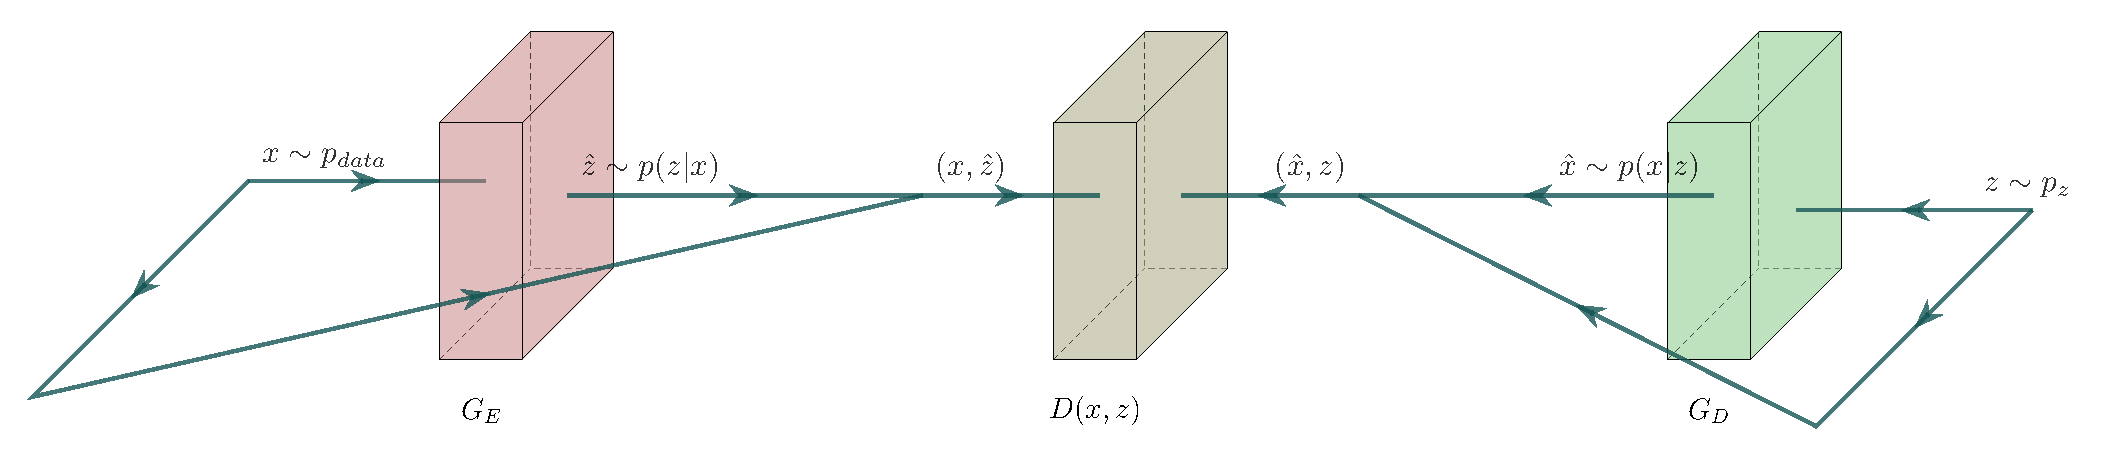
\includegraphics[width=.9\textwidth]{aligan}
    \caption{ALI architecture overview}
    \label{fig:aligan_model}
\end{figure}

AliGAN architecture is depicted as a generator and a discriminator in Figure \ref{fig:aligan_model}.
Significant change in ALI is that the generator is the combination of decoder network $G_D$ and an
encoder network $G_E$. Encoder network represents the joint distribution $p_{E}(x, z)$ which has the marginal
$p_{\text{data}(x)}$ and decoder network represents the joint distribution $p_{D}(x, z)$ with the marginal
$p_z(z)$ which represents the factorized noise distribution ( $\mathcal{N}(0, 1)$). The
objective function of the ALI is to match these two joint distributions. Successing in this goal
also ensures the match of marginals and conditional distributions $p(z | x)$ and $p(x | z)$
. Discriminator $D(x,z)$ is also modified to support this new objective function. It is trained to
distinguish between the joint pairs  $(x, \hat{z} = G_{E}(x))$ and $(\hat{x} = G_{D}(z), z)$ as data
and noise.

\begin{figure}[h!]
	\centering
	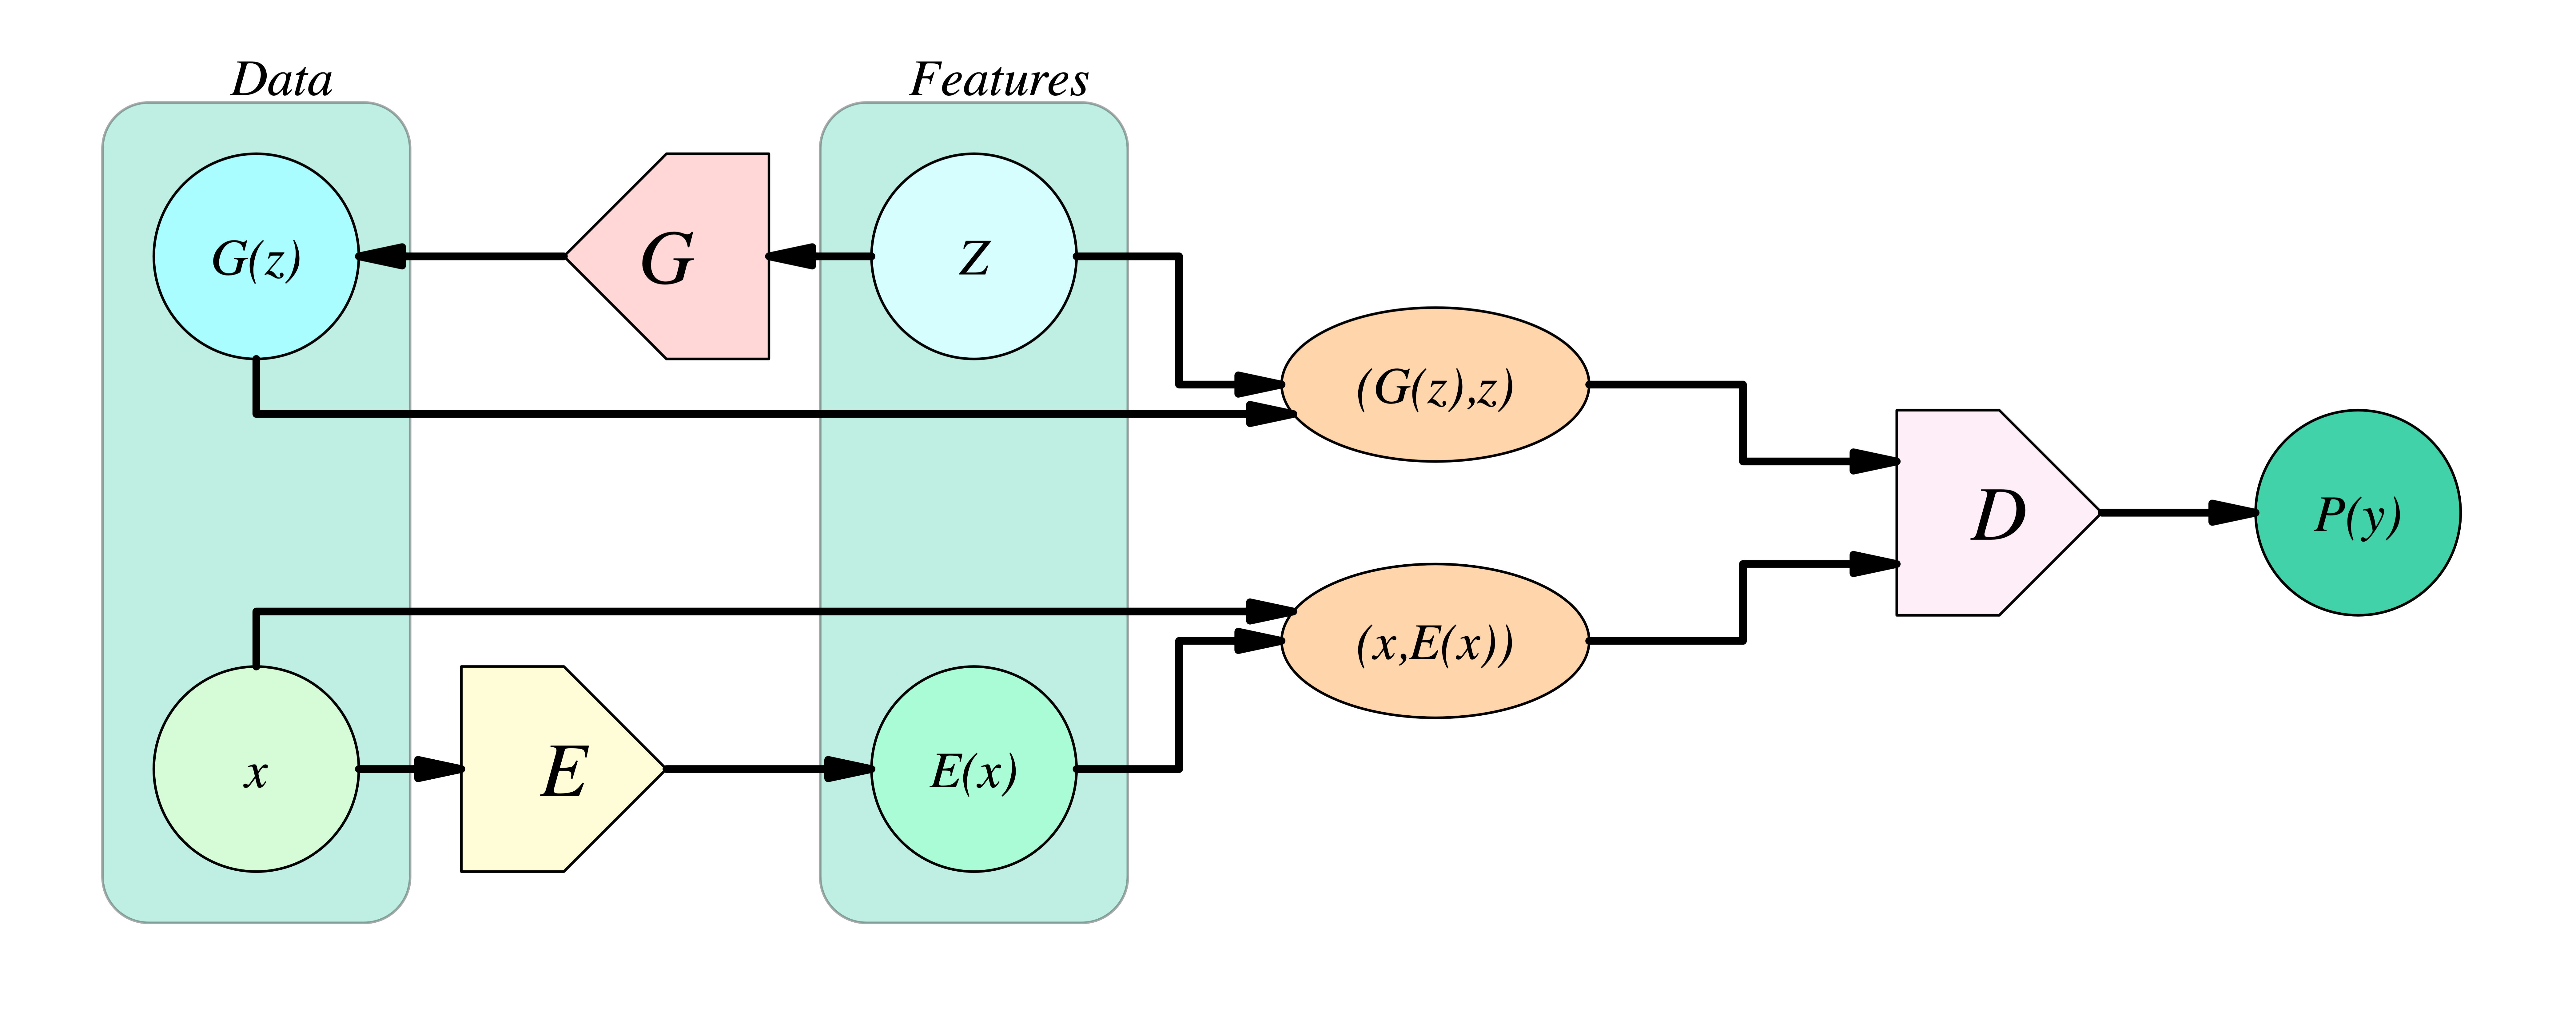
\includegraphics[width=.9\textwidth]{bigan}
    \caption{BiGAN architecture overview}
    \label{fig:bigan_model}
\end{figure}


BiGAN architecture model is presented in Figure \ref{fig:bigan_model}. The architectures are
theoretically identical with the exception of the encoder network choice in practise. BiGAN
experiments are conducted with a deterministic network whilst ALI framework used a stochastic
network. Apart from the generator, BiGAN also trains the encoder network in an adversarial manner.
Same objective function used in GAN provides the relationship between the generator and encoder that
$G = E^{-1}$ and vice versa. This invertibility is the key aspect of the model and other
frameworks to provide an efficient inference with reliable sampling. We Know from the Section
\ref{sec:gan} that: 
$$
G : \Omega_{z} \mapsto \Omega_{x}
$$

We define the Encoder $E$ with reverse of that mapping:
$$
E : \Omega_{x} \mapsto \Omega_{z}
$$

Since this framework accepts the networks as deterministic we also redefine the distributions for
generator and encoder networks:
\begin{align*}
    p_G(x | z) & = \delta (x - G(z)) \\
    p_E(z | x) & = \delta (z - E(x))
\end{align*}

The objective function of the framework can be characterized as:
\begin{equation}
    \min _{G, E} \max _{D} V(D, E, G)
\end{equation}
 
where
\begin{multline}
    \label{eqn:bigan_v}
V(D, E, G) :=\mathbb{E}_{\mathbf{x} \sim p_{\mathbf{X}}}  \underbrace{\left[ \mathbb{E}_{\mathbf{z} \sim p_{E}(\cdot | \mathbf{x})}[\log D(\mathbf{x}, \mathbf{z})] \right]}_{\log D(\mathbf{x}, E(\mathbf{x}))} + \\ \mathbb{E}_{\mathbf{z} \sim p_{\mathbf{Z}}} \underbrace{  \left[ \mathbb{E}_{\mathbf{x} \sim p_{G}(\cdot | \mathbf{z})}[\log (1-D(\mathbf{x}, \mathbf{z}))] \right]}_{\log (1-D(G(\mathbf{z}), \mathbf{z}))}
\end{multline}

To prove that the encoder is the inverse of the generator, optimal discriminator needs to be
determined \cite{Donahue2017AdversarialFL}. Joint distributions of the generator and encoder can
be illustrated as the marginals of the data and noise and related conditional probability
distributions. Here $p_{X}(x)$ represents the probability distribution of the training data and $p_{Z}$ 
represents the latent noise distribution.
\begin{align}
    \label{eqn:bigan_gz}
    p_{GZ} (x, z ) &:= p_G(x | z) p_{Z} (z) \\[5pt] 
    \label{eqn:bigan_ex}
    p_{EX} (x, z ) &:= p_E(z | x) p_{X} (x) 
\end{align}

The joint latent space and image space for the problem can also be illustrated as a joint
representation.
$$
\Omega := \Omega_{X} \times \Omega_{Z}
$$

For the region $R \subseteq \Omega$ probability
measures \cite{RePEc:eee:csdana:v:20:y:1995:i:6:p:703-702} of encoder and generator is defined in
Equation \ref{eqn:prob_measure1} and \ref{eqn:prob_measure2} respectively \cite{Donahue2017AdversarialFL}.

 \begin{align}
    \begin{split}\label{eqn:prob_measure1}
    P_{E \mathbf{X}}(R)  :={}&\int_{\Omega} p_{E \mathbf{X}}(\mathbf{x}, \mathbf{z})
    \mathbf{1\footnotemark}_{[(\mathbf{x}, \mathbf{z}) \in R]} \mathrm{d}(\mathbf{x}, \mathbf{z})= \\ 
    & \quad \int_{\Omega \mathbf{x}} p_{\mathbf{X}}(\mathbf{x}) \int_{\Omega \mathbf{z}} p_{E}(\mathbf{z} | \mathbf{x})
    \mathbf{1}_{[(\mathbf{x}, \mathbf{z}) \in R]} \mathrm{d} \mathbf{z} \mathrm{d} \mathbf{x}       
    \end{split}\\
    {}&=\int_{\Omega_{\mathbf{X}}} p_{\mathbf{X}}(\mathbf{x})\left(\int_{\Omega_{\mathbf{Z}}} \delta(\mathbf{z}-E(\mathbf{x})) \mathbf{1}_{[(\mathbf{x}, \mathbf{z}) \in R]} \mathrm{d} \mathbf{z}\right) \mathrm{d} \mathbf{x} \\[5pt]
    {}& =\int_{\Omega_{\mathbf{X}}} p_{\mathbf{X}}(\mathbf{x}) \mathbf{1}_{[(\mathbf{x}, E(\mathbf{x})) \in R]} \mathrm{d} \mathbf{x} \\[5pt]
    \begin{split}\label{eqn:prob_measure2}
    P_{G \mathbf{Z}}(R) :={}&\int_{\Omega} p_{G \mathbf{Z}}(\mathbf{x}, \mathbf{z}) 
    \mathbf{1}_{[(\mathbf{x},\mathbf{z}) \in R]} \mathrm{d}(\mathbf{x}, \mathbf{z})= \\ 
    & \quad \int_{\Omega_{\mathbf{Z}}} p_{\mathbf{Z}}(\mathbf{z}) \int_{\Omega_{\mathbf{X}}} p_{G}(\mathbf{x} | \mathbf{z})
    \mathbf{1}_{[(\mathbf{x}, \mathbf{z}) \in R]} \mathrm{d} \mathbf{x} \mathrm{d} \mathbf{z} 
    \end{split}\\
    {}&=\int_{\Omega_{\mathbf{Z}}} p_{\mathbf{Z}}(\mathbf{z})\left(\int_{\Omega_{\mathbf{X}}} \delta(\mathbf{x}-G(\mathbf{z})) \mathbf{1}_{[(\mathbf{x}, \mathbf{z}) \in R]} \mathrm{d} \mathbf{x}\right) \mathrm{d} \mathbf{z} \\[5pt]
    {}& =\int_{\Omega_{\mathbf{Z}}} p_{\mathbf{Z}}(\mathbf{z}) \mathbf{1}_{[(G(\mathbf{z}), \mathbf{z}) \in R]} \mathrm{d} \mathbf{z}
\end{align}        
\footnotetext{ Indicator function is a type of characteristic function that is used to indicate a
membership on a subset $X$. It is denoted with bold \textbf{1} symbol.}  

Probability measures over regions on the image data $R_X \subseteq \Omega_{X}$ and the latent noise
$R_Z \subseteq \Omega_{Z}$ can be similarly defined.

\begin{align}
    P_{\mathbf{X}}\left(R_{\mathbf{X}}\right) :=&\int_{\Omega_{\mathbf{X}}} p_{\mathbf{X}}(\mathbf{x}) \mathbf{1}_{\left[\mathbf{x} \in R_{\mathbf{X}}\right]} \mathrm{d} \mathbf{x} \\[5pt]
    P_{\mathbf{X}}\left(R_{\mathbf{X}}\right) :=&\int_{\Omega_{\mathbf{X}}} p_{\mathbf{X}}(\mathbf{x}) \mathbf{1}_{\left[\mathbf{x} \in R_{\mathbf{X}}\right]} \mathrm{d} \mathbf{x}
\end{align}

Optimal discriminator follows the same derivation from the GAN framework
\cite{Goodfellow:2014:GAN:2969033.2969125}. The Objective Equation \ref{eqn:bigan_v} can be reduced
to the Jensen-Shannon divergence between joint distributions $P_{E\mathbf{X}}$ and $P_{G\mathbf{Z}}$
with the proof of following propositions from the BiGAN \cite{Donahue2017AdversarialFL}.

\begin{prop}
    \label{prop:bigan_1}
    For any $E$ and $G$, the optimal discriminator $D^*_{EG} := \\ \underset{D}{\text{argmax}}  V(D, E,
    G)$ is the Radon-Nikodym derivative $f_{EG} := \frac{dP_{E\mathbf{X}}}{dP_{E\mathbf{X}} +
    dP_{G\mathbf{Z}}}  : \Omega  \mapsto [0, 1]$ of measure $P_{E\mathbf{X}}$ with respect to measure
    $ dP_{E\mathbf{X}} + dP_{G\mathbf{Z}}$.
\end{prop}

\begin{prop}
    \label{prop:bigan_2}
  The encoder and generator's objective for an optimal discriminator $C(E, G):= \underset{D}{max}
  V(D, E, G) = V(D^*_{EG}, E, G)$ can be rewritten in terms of the Jensen-Shannon divergence between
  the measures $P_{EX}$ and $P_{GZ}$ as $C(E, G) = 2 D_{JS} (P_{E\mathbf{X}} \parallel P_{G\mathbf{Z}}) -
  \log 4$    
\end{prop}

Discriminator is trained with both the encoder and generator network output. Authors of \cite{Donahue2017AdversarialFL}
suggests that it is rational to assume that if we were to define a probability measure for discriminator using 
probability measures of both networks. So we let $P_{EG}$
be the average of $P_{E\mathbf{X}}$ and $P_{G\mathbf{Z}}$. 
\begin{equation}
  P_{EG} = \frac{P_{E\mathbf{X}} + P_{G\mathbf{Z}}}{2}  
\end{equation}

Since both $P_{E\mathbf{X}}$ and $P_{G\mathbf{Z}}$ are continuous with respect to the $P_{EG}$, the
relationship of RN derivatives of $f_{EG}$ and $f_{GE}$ is defined accordingly:
\begin{align}
  f_{EG} :=& \frac{ d P_{E\mathbf{X}} }{ d P_{E\mathbf{X}} + d P_{G\mathbf{Z}}} \\[5pt]
  f_{GE} :=& \frac{ d P_{G\mathbf{Z}} }{ d P_{E\mathbf{X}} + d P_{G\mathbf{Z}}} \\[5pt]
  f_{EG} + f_{GE} :=   \frac{ d P_{G\mathbf{Z}} }{ d P_{E\mathbf{X}} + d P_{G\mathbf{Z}}} &+ \frac{ d P_{E\mathbf{X}} }{ d P_{E\mathbf{X}} + d P_{G\mathbf{Z}}} = \frac{ d( P_{G\mathbf{Z}} + P_{E\mathbf{X}}) }{ d( P_{G\mathbf{Z}} + P_{E\mathbf{X}} ) } = 1 
\end{align}

Using the property of RN derivative (Equation \ref{eqn:radon}) we can transform the expected value
function and rewrite the objective function of the BiGAN with a single probability
measure \cite{Donahue2017AdversarialFL} \cite{Goodfellow:2014:GAN:2969033.2969125}.
\begin{equation}
    \label{eqn:transform}
    \mathbb{E}_{\mathbf{x} \sim P}[g(\mathbf{x})]=\int_{\Omega} g \mathrm{d} P=\int_{\Omega} g \frac{\mathrm{d} P}{\mathrm{d} Q} \mathrm{d} Q=\int_{\Omega} g f_{P Q} \mathrm{d} Q=\mathbb{E}_{\mathbf{x} \sim Q}\left[f_{P Q}(\mathbf{x}) g(\mathbf{x})\right]
    %\caption{expression change of expected value computation with a different distribution}
\end{equation}
We start by rewriting the original objective function with the joint probability distributions.
\begin{equation}
    V(D, E, G) = \mathbb{E}_{(\mathbf{x}, \mathbf{z}) \sim P_{E \mathbf{X}}}[\log D(\mathbf{x}, \mathbf{z})]+\mathbb{E}_{(\mathbf{x}, \mathbf{z}) \sim P_{G \mathbf{Z}}}[\log (1-D(\mathbf{x}, \mathbf{z}))] 
\end{equation}

Then the transformation described in Equation \ref{eqn:transform} is applied.
\begin{equation}
    =\mathbb{E}_{(\mathbf{x}, \mathbf{z}) \sim P_{E G}}  [ \underbrace{2 f_{E G}}_{\frac{\mathrm{d} P_{E X}}{\mathrm{d} P_{E G}}}(\mathbf{x}, \mathbf{z}) \log D(\mathbf{x}, \mathbf{z})] +\mathbb{E}_{(\mathbf{x}, \mathbf{z}) \sim P_{E G}}[\underbrace{2 f_{G E}}_{\frac{\mathrm{d} P_{G Z}}{\mathrm{d} P_{E G}}}(\mathbf{x}, \mathbf{z}) \log (1-D(\mathbf{x}, \mathbf{z}))]
\end{equation}

The final stage of the Equation \ref{eqn:bigan_complete_2} falls into a type of function $ f(a,y) = a\log y + (1 -a) \log(1-y)$
\cite{Donahue2017AdversarialFL} which provides $\underset{y}{argmax} f(a,y) = a\ \text{ for any }\ a
\in [0,1]$. Thus the optimal Discriminator $D^*_{EG} = f_{EG}$. That proves the first proposition. 
\begin{align}
    &=2 \mathbb{E}_{(\mathbf{x}, \mathbf{z}) \sim P_{E G}}\left[f_{E G}(\mathbf{x}, \mathbf{z}) \log D(\mathbf{x}, \mathbf{z})+f_{G E}(\mathbf{x}, \mathbf{z}) \log (1-D(\mathbf{x}, \mathbf{z}))\right] \\[5pt]
    \label{eqn:bigan_complete_2}
    &=2 \mathbb{E}_{(\mathbf{x}, \mathbf{z}) \sim P_{E G}}\left[f_{E G}(\mathbf{x}, \mathbf{z}) \log D(\mathbf{x}, \mathbf{z})+\left(1-f_{E G}(\mathbf{x}, \mathbf{z})\right) \log (1-D(\mathbf{x}, \mathbf{z}))\right]
\end{align}

Second proposition can be proved with the same approach from
GAN \cite{Goodfellow:2014:GAN:2969033.2969125} using the connection acquired from the first
proposition \cite{Donahue2017AdversarialFL}.

First the objective equation is rewritten with the optimal discriminator and its equivalent RN
derivative \cite{Donahue2017AdversarialFL}.
\begin{align}
    C(E, G)=&\max _{D} V(D, E, G)=V\left(D_{E G}^{*}, E, G\right) \\[5pt]
    & =\mathbb{E}_{(\mathbf{x}, \mathbf{z}) \sim P_{E \mathbf{X}}}\left[\log D_{E G}^{*}(\mathbf{x}, \mathbf{z})\right]+\mathbb{E}_{(\mathbf{x}, \mathbf{z}) \sim P_{G \mathbf{Z}}}\left[\log \left(1-D_{E G}^{*}(\mathbf{x}, \mathbf{z})\right)\right] \\[5pt]
    & =\mathbb{E}_{(\mathbf{x}, \mathbf{z}) \sim P_{E \mathbf{X}}}\left[\log f_{E G}(\mathbf{x}, \mathbf{z})\right]+\mathbb{E}_{(\mathbf{x}, \mathbf{z}) \sim P_{G \mathbf{Z}}}\left[\log f_{G E}(\mathbf{x}, \mathbf{z})\right]
\end{align}

Then addition - subtraction of $\log4$ is applied following the Equation \ref{eqn:gan_optim_proof}
to interpret the result as Jensen-Shannon divergence, hence proving the second proposition.
\begin{align}
    &=\mathbb{E}_{(\mathbf{x}, \mathbf{z}) \sim P_{E \mathbf{X}}}\left[\log \left(2 f_{E G}(\mathbf{x}, \mathbf{z})\right)\right]+\mathbb{E}_{(\mathbf{x}, \mathbf{z}) \sim P_{G} \mathbf{z}}\left[\log \left(2 f_{G E}(\mathbf{x}, \mathbf{z})\right)\right]-\log 4 \\[5pt]
    & =\mathrm{D}_{\mathrm{KL}}\left(P_{E \mathbf{X}} \| P_{E G}\right)+\mathrm{D}_{\mathrm{KL}}\left(P_{G \mathbf{Z}} \| P_{E G}\right)-\log 4 \\[5pt]
    &=\mathrm{D}_{\mathrm{KL}}\left(P_{E \mathbf{X}}| | \frac{P_{E \mathbf{X}}+P_{G \mathbf{Z}}}{2}\right)+\mathrm{D}_{\mathrm{KL}}\left(P_{G \mathbf{Z}}| | \frac{P_{E \mathbf{X}}+P_{G \mathbf{Z}}}{2}\right)-\log 4 \\[5pt]
    & =2 \mathrm{D}_{\mathrm{JS}}\left(P_{E \mathbf{X}} \| P_{G \mathbf{Z}}\right)-\log 4 . \square
\end{align}

Proposition \ref{prop:bigan_2} allows us to characterize the objective function of the BiGAN in
terms of the Jensen-Shannon divergence but implicitly it proves just like in Equation
\ref{eqn:gan_eqaul} that the global minimum of the training criterion is only achieved with the
equality of the probability measures $P_{E\mathbf{X}}$ and $P_{G\mathbf{Z}}$. Consequentially this
gives the optimal condition for both encoder and generator. 

\begin{theorem}
    \label{th:bigan_inv}
    if $E$ and $G$ are an optimal encoder and generator, then $E = G^{-1}$ almost everywhere; that is,
    $G(E(x)) = x$ for $P_X$ almost every $x \in \Omega_x$, and $E(G(z)) = z$ for $P_z$, almost every
    $z \in \Omega_z$ \text{\cite{Donahue2017AdversarialFL}}.
\end{theorem}

The inversion property of the BiGAN framework is dependent on the factor of $P_{E\mathbf{X}}$ being
equal to $P_{G\mathbf{Z}}$ in the optimal state. Let $R_{X}^{0}$ be the region that
reconstructed image from the encoded noise is not equal to the input image and let $R^{0}$ be the
region for the data, noise pairs which the data is also a member of the $R^{0}_{X}$. Using the
optimal encoder and decoder, it can be proven that the probability measure for the region
$R^{0}_{X}$ is zero, meaning that for almost every $x$ in the region $\Omega_x$, $G(E(x)) = x$ and
vice versa.

\begin{align}
    R^{0}_{X} :=& \{x \in \Omega_x : x \neq G(E(x))\} \\[5pt]
    R^{0} :=& \{(x,z) \in \Omega : \mathbf{z} = E(x) \land x \in R^{0}_{X}\}\\[5pt]
    P_{\mathbf{X}}\left(R_{\mathbf{X}}^{0}\right) &=\int_{\Omega_{\mathbf{X}}} p_{\mathbf{X}}(\mathbf{x}) \mathbf{1}_{\left[\mathbf{x} \in R_{\mathbf{x}}^{0}\right.} ] \mathrm{d} \mathbf{x} \\[5pt]
    &=\int_{\Omega_{\mathbf{X}}} p_{\mathbf{X}}(\mathbf{x}) \mathbf{1}_{\left[(\mathbf{x}, E(\mathbf{x})) \in R^{0}\right]} \mathrm{d} \mathbf{x} \\[5pt]
    & =P_{E \mathbf{X}}\left(R^{0}\right)\\[5pt]
    & =P_{G \mathbf{Z}}\left(R^{0}\right)\\[5pt]
    & =\int_{\Omega_{\mathbf{Z}}} p_{\mathbf{Z}}(\mathbf{z}) \mathbf{1}_{\left[(G(\mathbf{z}), \mathbf{z}) \in R^{0}\right]} \mathrm{d} \mathbf{z}\\[5pt]
    & =\int_{\Omega_{\mathbf{Z}}} p_{\mathbf{Z}}(\mathbf{z}) \mathbf{1}\left[\mathbf{z}=E(G(\mathbf{z})) \wedge G(\mathbf{z}) \in R_{\mathbf{X}}^{0}\right] \mathrm{d} \mathbf{z}\\[5pt]
    & =\int_{\Omega_{\mathbf{Z}}} \underbrace{p_{\mathbf{Z}}(\mathbf{z}) \quad \mathbf{1}_{[\mathbf{z}=E(G(\mathbf{z})) \wedge G(\mathbf{z}) \neq G(E(G(\mathbf{z})))]}}_{=0 \text { for any } \mathbf{z}, \text { as } \mathbf{z}=E(G(\mathbf{z})) \Longrightarrow G(\mathbf{z})=G(E(G(\mathbf{z})))} \mathrm{d} \mathbf{z}\\[5pt]
    &= 0. \square  \\[5pt]
\end{align}

Training of BiGAN framework is implemented using the same adversarial process of GANs. Encoder and
generator network are trained together since they both try to minimize the objective. Each iteration
is divided into two parts. First the discriminator is trained using the outputs from the encoder and
generator with fixed weights, pushing the gradient of the function towards a positive step. Also the
parameters of discriminator $\theta_D$ is updated. Then $\theta_E$ and $\theta_G$ the parameters of
encoder and generator are updated concurrently with a negative direction in the gradient of the
objective function \cite{Donahue2017AdversarialFL}.

Loss functions for the training optimization and anomaly score computation differs from AnoGAN\cite{Schlegl2017UnsupervisedAD}. 
AnoGAN framework uses the
combination of the reconstruction loss (Equation \ref{eqn:anogan_rl}) and the discrimination loss
(Equation \ref{eqn:anogan_dl}) both to infer $z$ from the query image and to compute the anomaly
score. BiGAN framework's encoder is trained with the kind of function that is used to train the
generator, sigmoid cross entropy. The advantage of the BiGAN is the reduced inference time to
compute the anomaly score because the inferred noise from the query image $\hat{x}$ is the output
from the generator $\hat{z} = E(\hat{x})$. 

Anomaly score computation of BiGAN however, is the same approach used in AnoGAN. It uses a
combination of the discriminaton loss and a reconstruction loss. The degree of norms used in the
computation differs in the experiment stage to observe the behavior of the anomaly score.
Anomalous samples of the test dataset is determined by accepting the anomaly score that is greater
then a predetermined cut-off value. This value varies depending on the type of dataset and the dimensional
complexity of the dataset the framework trained on.
% model implementation -> Later
The implementation of this model contains the same generator and discriminator implementations as AnoGAN model.
Details of the architecture can be found in the appendix Section. (see Section \ref{app:bigan})

\subsection{ALAD}
\label{sec:alad}

Adversarially Learned Anomaly Detection, or ALAD \cite{DBLP:journals/corr/abs-1812-02288} is a
framework designed for the anomaly detection task. It builds upon the idea of AnoGAN, using the base
architecture from the AliGAN and BiGAN with additional improvements incorporated to increase the
stabilization of the adversarial training in both  discriminator network and encoder, generator network pairs.
I will first describe the improvements introduced to the adversarial training framework and discuss
their potential advantages over the previous approach. Then I will explain the ALAD architecture in
detail. Lastly, learning of the model and anomaly score computation choices will be discussed. 

\subsubsection{Spectral Normalization}
\label{sec:alad_sn}

Even tough the training of GAN works in practice, it may easily become unstable in certain
conditions. For example, in high dimensional space, density ratio estimation of the discriminator
network is often inaccurate and this results in generator networks fail to learn the dimensional
structure of the target data distribution \cite{methods}. Consequently, when the support of the model
distribution and the target distribution is disjoint, then the discriminator may become decently
efficient classifying real data from the generated data sample. In this scenario, the generator
fails to learn to improve sample fake image data. Spectral Normalization is one of the recent
proposed improvement methods to stabilize the weights of the discriminator network by bounding its
gradients using Lipschitz continuity \cite{inproceedings_sn}. 

Consider the optimal discriminator of $D(\boldsymbol{x}, \theta)=\mathcal{A}(f(\boldsymbol{x}, \theta))$ in equation \ref{eqn:opt_d}. It takes the form :
\begin{multline}
    D_{G}^{*}(\boldsymbol{x})=\frac{q_{\text { data }}(\boldsymbol{x})}{q_{\text { data }}(\boldsymbol{x})+p_{G}(\boldsymbol{x})}=\operatorname{sigmoid}\left(f^{*}(\boldsymbol{x})\right), \\ \text { where } f^{*}(\boldsymbol{x})=\log q_{\text { data }}(\boldsymbol{x})-\log p_{G}(\boldsymbol{x}) 
\end{multline}

Where $\mathcal{A}$ is an activation function corresponding to the divergence of distance measure of the
user’s choice (usually a sigmoid). With the derivative of: 

\begin{equation}
    \nabla_{\boldsymbol{x}} f^{*}(x)=\frac{1}{q_{\mathrm{data}}(\boldsymbol{x})} \nabla_{\boldsymbol{x}} q_{\mathrm{data}}(\boldsymbol{x})-\frac{1}{p_{G}(\boldsymbol{x})} \nabla_{\boldsymbol{x}} p_{G}(\boldsymbol{x})  
\end{equation}

This gradient function can be unbounded or even incomputable depending on the distribution. Spectral
normalization is applied to introduce regularity condition to derivative $f(\boldsymbol{x})$
\cite{inproceedings_sn}.

Discriminator function can be modified to apply this regularization to the objective function: 
\begin{equation}
\begin{array}{l}{\text { arg max } V(G, D)} \\ {\|f\|_{\mathrm{Lip}} \leq K}\end{array} 
\end{equation}

Where $\|f\|_{\mathrm{Lip}}$ is depicted as the smallest value $M$ such that: 

\begin{equation}
    \left\|f(\boldsymbol{x})-f\left(\boldsymbol{x}^{\prime}\right)\right\| /\left\|\boldsymbol{x}-\boldsymbol{x}^{\prime}\right\| \leq M 
\end{equation}
for any $x$, $x'$ with the norm being the $l_2$ norm. $x$ in $X$,\cite{sohrab2011basic}

Using the computation of the K-Lipschitz function of the each layer in discriminator, the spectral
norm of each layer weight matrix can be normalized so the updated weights of the discriminator after
each epoch of training becomes:

\begin{equation}
    \overline{W}_{\mathrm{SN}}(W) :=W / \sigma(W) 
\end{equation}

Overall implementation of the spectral normalization addition to batch normalization proved useful for the performance of 
ALAD, particularly in the stabilization of the discriminator training. Model also employed this reparameterization in their 
architecture as well. 

\subsubsection{Conditional Entropy (ALICE Framework)}
\label{sec:alad_alice}

The BiGAN framework in Section \ref{sec:bigan} aims to learn both the mapping from the input image
data to a latent representation with its encoder module and the inverse of that mapping relation
with its generator network. It acquires these mappings by training its encoder and generator networks
together in an adversarial manner to learn a joint distribution depicted in Equation
\ref{eqn:bigan_ex} and \ref{eqn:bigan_gz}. Problem suggested by the ALICE
framework\cite{Li2017TowardsUA} is that learning the joint distribution alone doesn't help the model
to reconstruct images necessarily faithful to the reproductions of the input data
\cite{Li2017TowardsUA}. This is because the objective function is built only to match joint
distributions of image and noise pairs at the same time potential dependency structures or
correlations between two random variables within each joint representation is not specified or
constrained \cite{Li2017TowardsUA}.

In order to reduce identifiable issues associated with the objective of BiGAN, the
conditionals $P_{G}(x|z)$ and $P_{E}(z|x)$ needs to be constrained and be under supervision using a
paired samples from the domain $\Omega_{x}$ and $\Omega_{z}$. Information-theoretic measure
conditional entropy is used to provide this regularization. 

Conditional entropy quantifies the amount of information needed to describe the outcome of a random variable 
$Y$ given that the value of another random variable $X$ is known \cite{Cover:2006:EIT:1146355}  under the joint distribution 
$$
\pi(x ,y ) ,\quad x \in X , y \in Y
$$ 
For the BiGAN framework conditional entropies are defined below:

\begin{align}
    H^{\pi}(\boldsymbol{x} | \boldsymbol{z}) \triangleq-\mathbb{E}_{\pi(\boldsymbol{x}, \boldsymbol{z})}[\log \pi(\boldsymbol{x} | \boldsymbol{z})] \\[5pt]
    H^{\pi}(\boldsymbol{z} | \boldsymbol{x}) \triangleq-\mathbb{E}_{\pi(\boldsymbol{x}, \boldsymbol{z})}[\log \pi(\boldsymbol{z} | \boldsymbol{x})] 
\end{align}

The Conditional entropy defined above is dependent on the underlying distribution of the random
variables, in this case the probability distributions learned by the encoder and generator networks $p_{G}(x)$ and
$p_{E}(z)$. In practice this value is intractable because we don't have access to the saddle points
of the objective function beforehand. As an alternative, the approximation of the conditional
entropy is calculated by bounding conditional entropy to the criterion of cycle-consistency \cite{Zhu2017UnpairedIT}.

Cycle consistency is the similarity of the reconstruction to the input data. Denoting the
reconstruction of $x$ as $x'$, the cycle can be defined as: 

\begin{equation}
  x' = G(z'), \quad z' = E(x),\quad x \in \Omega_{x},\quad x' \approx G(E(x)) 
\end{equation}

In other GAN frameworks like Cycle-GAN\cite{Zhu2017UnpairedIT}, Disco-GAN \cite{Kim2017LearningTD}
and Dual-GAN \cite{Yi2017DualGANUD} cycle consistency constraint is implemented leveraging
$\ell_{k}$ losses with $k=1,2$. Using $\ell_2$ based pixel-wise loss functions to reconstruct the samples
leads to blurry images during inference \cite{Larsen2016AutoencodingBP}\cite{Li2017TowardsUA}.
To enforce a better constraint and to improve the quality of the reconstructed samples, this
framework suggests using the feature layer of the discriminator to compute the loss for the
conditional entropy constraint. Objective function to approximate this constraint is given
below:
\begin{multline}
    \label{eqn:alice}
     \min _{\boldsymbol{E}, \boldsymbol{G}} \max _{\boldsymbol{D}}
\mathcal{L}_{\mathrm{Cycle}}(E,G,D)
=\mathbb{E}_{\boldsymbol{x} \sim p_{\text{data}}(\boldsymbol{x})}\left[\log
\sigma\left(f_{\boldsymbol{D}}(\boldsymbol{x}, \boldsymbol{x})\right)\right] \\
+\mathbb{E}_{\hat{\boldsymbol{x}} \sim p_{\boldsymbol{G}}(\hat{\boldsymbol{x}} | \boldsymbol{z}),
\boldsymbol{z} \sim p_{\boldsymbol{E}}(\boldsymbol{z} | \boldsymbol{x})} \log
\left(1-\sigma\left(f_{\boldsymbol{D}}(\boldsymbol{x}, \hat{\boldsymbol{x}})\right)\right) ] 
\end{multline}

This additional adversarial training is implemented into the ALAD architecture to enforce a
constraint to improve the quality of reconstructed noise and the image. Its addition is explained in
the next section.

\subsubsection{ALAD Architecture}
\label{sec:alad_arc}

Training of the framework shares the same adversarial approach with BiGAN
( see Section \ref{sec:bigan}). Generator network simultaneously learns the mapping from input data to a latent
representation while the encoder network learns the opposite. Model also incorporates the mentioned
improvements to increase the stabilization of the training procedure. Architecture overview is
illustrated in Figure \ref{fig:alad_model}

\begin{figure}[h!]
	\centering
	\includegraphics[width=.9\textwidth]{alad}
    \caption{ALAD architecture overview}
    \label{fig:alad_model}
\end{figure}

Formally the ALAD architecture tries to match the joint distributions: 
\begin{equation}
    p_{E} (x, z) = p_{E}(z | x) p_{\text{data}}(x) \\[5pt]
    p_{G} (x, z) = p_{G}(x | z) p_{Z}(z)
\end{equation}

and tries the separate data, noise pairs $(x, E(x))$ and $(G(z), z)$ with an adversarial
discriminator network $D$. For this framework we refer to the main discriminator as $D_{xz}$. Main
objective function with the updated terms is :
\begin{equation}
\begin{aligned} V\left(D_{x z}, E, G\right) &=\mathbb{E}_{x \sim p_{\text{data}}}\left[\log D_{x z}(x, E(x))\right] \\ &+\mathbb{E}_{z \sim p_{Z}}\left[1-\log D_{x z}(G(z), z)\right]
 \end{aligned}
\end{equation}

Section \ref{sec:alad_alice} explains the convergence problem of the joint distribution. Because of
the lack of constraints imposed on the $p_{\text{data}}$ and $p_{Z}$, the objective function may not
converge properly and this consequentially decreases the quality of the reconstructed samples,
namely $x' \approx G(E(x))$. In addition to the image reconstruction, to enforce a constraint on the
noise encoding from the input image, $z' \approx (E(G(z)))$, ALAD model also adds a second
objective function to the overall adversarial training loop to regularize the conditional
distributions. Conditional Entropy term for the image and for the noise is defined below.
\begin{align}
    H^{\pi}(x | z)=-\mathbb{G}_{\pi(x, z)}[\log \pi(x | z)] \\[5pt]
    H^{\pi}(z | x)=-\mathbb{E}_{\pi(x, z)}[\log \pi(z | x)] 
\end{align}

As explained in the previous section, since the saddle points beforehand can't be obtained for the
computation, these terms can be approximated with the discriminators $D_{xx}$ and $D_{zz}$
respectively. Training of these discriminator networks is added to the main adversarial training loop as
a part of the discriminator network training. Their objective functions are defined in Equation
\ref{eqn:alad_discs}

\begin{align}
    \label{eqn:alad_discs}
\begin{split} V\left(D_{x x}, E, G\right) ={}&\mathbb{E}_{x \sim p_{\text{data}}}\left[\log D_{x x}(x, x)\right] \\ &+\mathbb{E}_{x \sim p_{\text{data}}}\left[1-\log D_{x x}(x, G(E(x)))\right] \end{split}  \\[5pt]
\begin{split} V\left(D_{z z}, E, G\right) ={}&\mathbb{E}_{z \sim p_{\mathcal{Z}}}\left[\log D_{z z}(z, z)\right] \\ &+\mathbb{E}_{z \sim p_{\mathcal{Z}}}\left[1-\log D_{z z}(z, E(G(z)))\right] \end{split}    
\end{align}

Putting it all together, ALAD framework solves the following combination of value function during the adversarial
training:
\begin{equation}
\begin{array}{l}{\min _{G, E} \max _{D_{x z}, D_{x x}, D_{z z}} V\left(D_{x z}, D_{x x}, D_{z z}, E, G\right)=} \\ {V\left(D_{x z}, E, G\right)+V\left(D_{x x}, E, G\right)+V\left(D_{z z}, E, G\right)}\end{array} 
\end{equation}

During the training, generator and encoder networks are updated simultaneously. In the
second part of the adversarial training iteration, all discriminators update their weights to both
regularize the reconstructions and to converge to equilibrium for the main value function. Spectral
normalization is used in every convolutional layer of the discriminators. Framework also implemented
them to the layers of encoder network with the purpose of further increasing the quality of the reconstructed
samples \cite{DBLP:journals/corr/abs-1812-02288}. The result of the training and its analysis will 
be discussed in Chapter \ref{chap:expres}.

The Anomaly score computation of the framework is based on the quality of the reconstructed query
samples. If the reconstructed query image is distant to the original input it will obtain a greater
anomaly score. ALAD framework suggests that because of the nature of the spatial data, even though
there are similarities, obtained noise during reconstruction may mask potential feature
similarities, preventing their detection. The suggested approach of the framework is to compute the
anomaly score using the feature layer of the $D_{xx}$ discriminator shown in Equation
\ref{eqn:alad_an}.
\begin{equation}
  \label{eqn:alad_an}
  A(x)=\left\|f_{x x}(x, x)-f_{x x}(x, G(E(x)))\right\|_{1} 
\end{equation}

In this equation, $f(\cdot, \cdot)$ represents the vector of activations of the layer before the
output of the $D_{xx}$ discriminator \cite{DBLP:journals/corr/abs-1812-02288}. Anomaly score
$A(\cdot)$ captures the confidence such that the given image is well encoded and reconstructed by
the generator and therefore it is from the real data distribution
\cite{DBLP:journals/corr/abs-1812-02288}. However different kinds of anomaly score computations are
also considered for the sake of comparison. 

These are (including the one discussed ):

\begin{equation}
\begin{aligned} \bullet L_{1} & : A(x)=\left\|x-x^{\prime}\right\|_{1} \\ \bullet L_{2} & : A(x)=\left\|x-x^{\prime}\right\|_{2} \\ \bullet \text { Logits } & : A(x)=\log \left(D_{x x}\left(x, x^{\prime}\right)\right) \\ \bullet \text { Features } & : A(x)=\left\|f_{x x}(x, x)-f_{x x}\left(x, x^{\prime}\right)\right\|_{1} \end{aligned}
\end{equation}

Overall this framework aims to improve the generator and encoder learning with improvements such as spectral
normalization and conditional entropy discriminators. Its performance with our dataset and ways to
improve the adversarial training will be discussed in Chapter \ref{chap:expres}.

\subsection{GANomaly \& Skip-GANomaly}

\label{sec:ganomaly}

GANomaly \cite{Akay2018GANomalySA} and Skip-GANomaly \cite{Akay2019SkipGANomalySC} are the
most recent models that focuses on the anomaly detection using adversarial training. 
Their performance on the benchmark datasets like CIFAR-10
\cite{cifar10} and SVHN \cite{Netzer2011ReadingDI} exceeds AnoGAN, BiGAN and ALAD. This
section will explain their structure and their differences in terms of one another.

GANomaly and Skip-Ganomaly models differ with a significant change in the model itself. Both 
models contain a generator and discriminator networks but generator network is actually composed of an
autoencoder network. Details of the both architecture will be discussed in order.

Generator network of the GANomaly framework composed of an encoder-decoder network as can be seen in
Figure \ref{fig:ganomaly_model}. The third network is the encoder network for the generated samples.
Generator network takes the image data as an input and sequentially it creates the latent
representation of the image and reconstruction from the latent representation then the second
encoder network encodes the latent representation of the reconstructed sample. Discriminator network
shares the same functionality as in GAN framework \cite{Goodfellow:2014:GAN:2969033.2969125}.
\begin{figure}[h!]
	\centering
	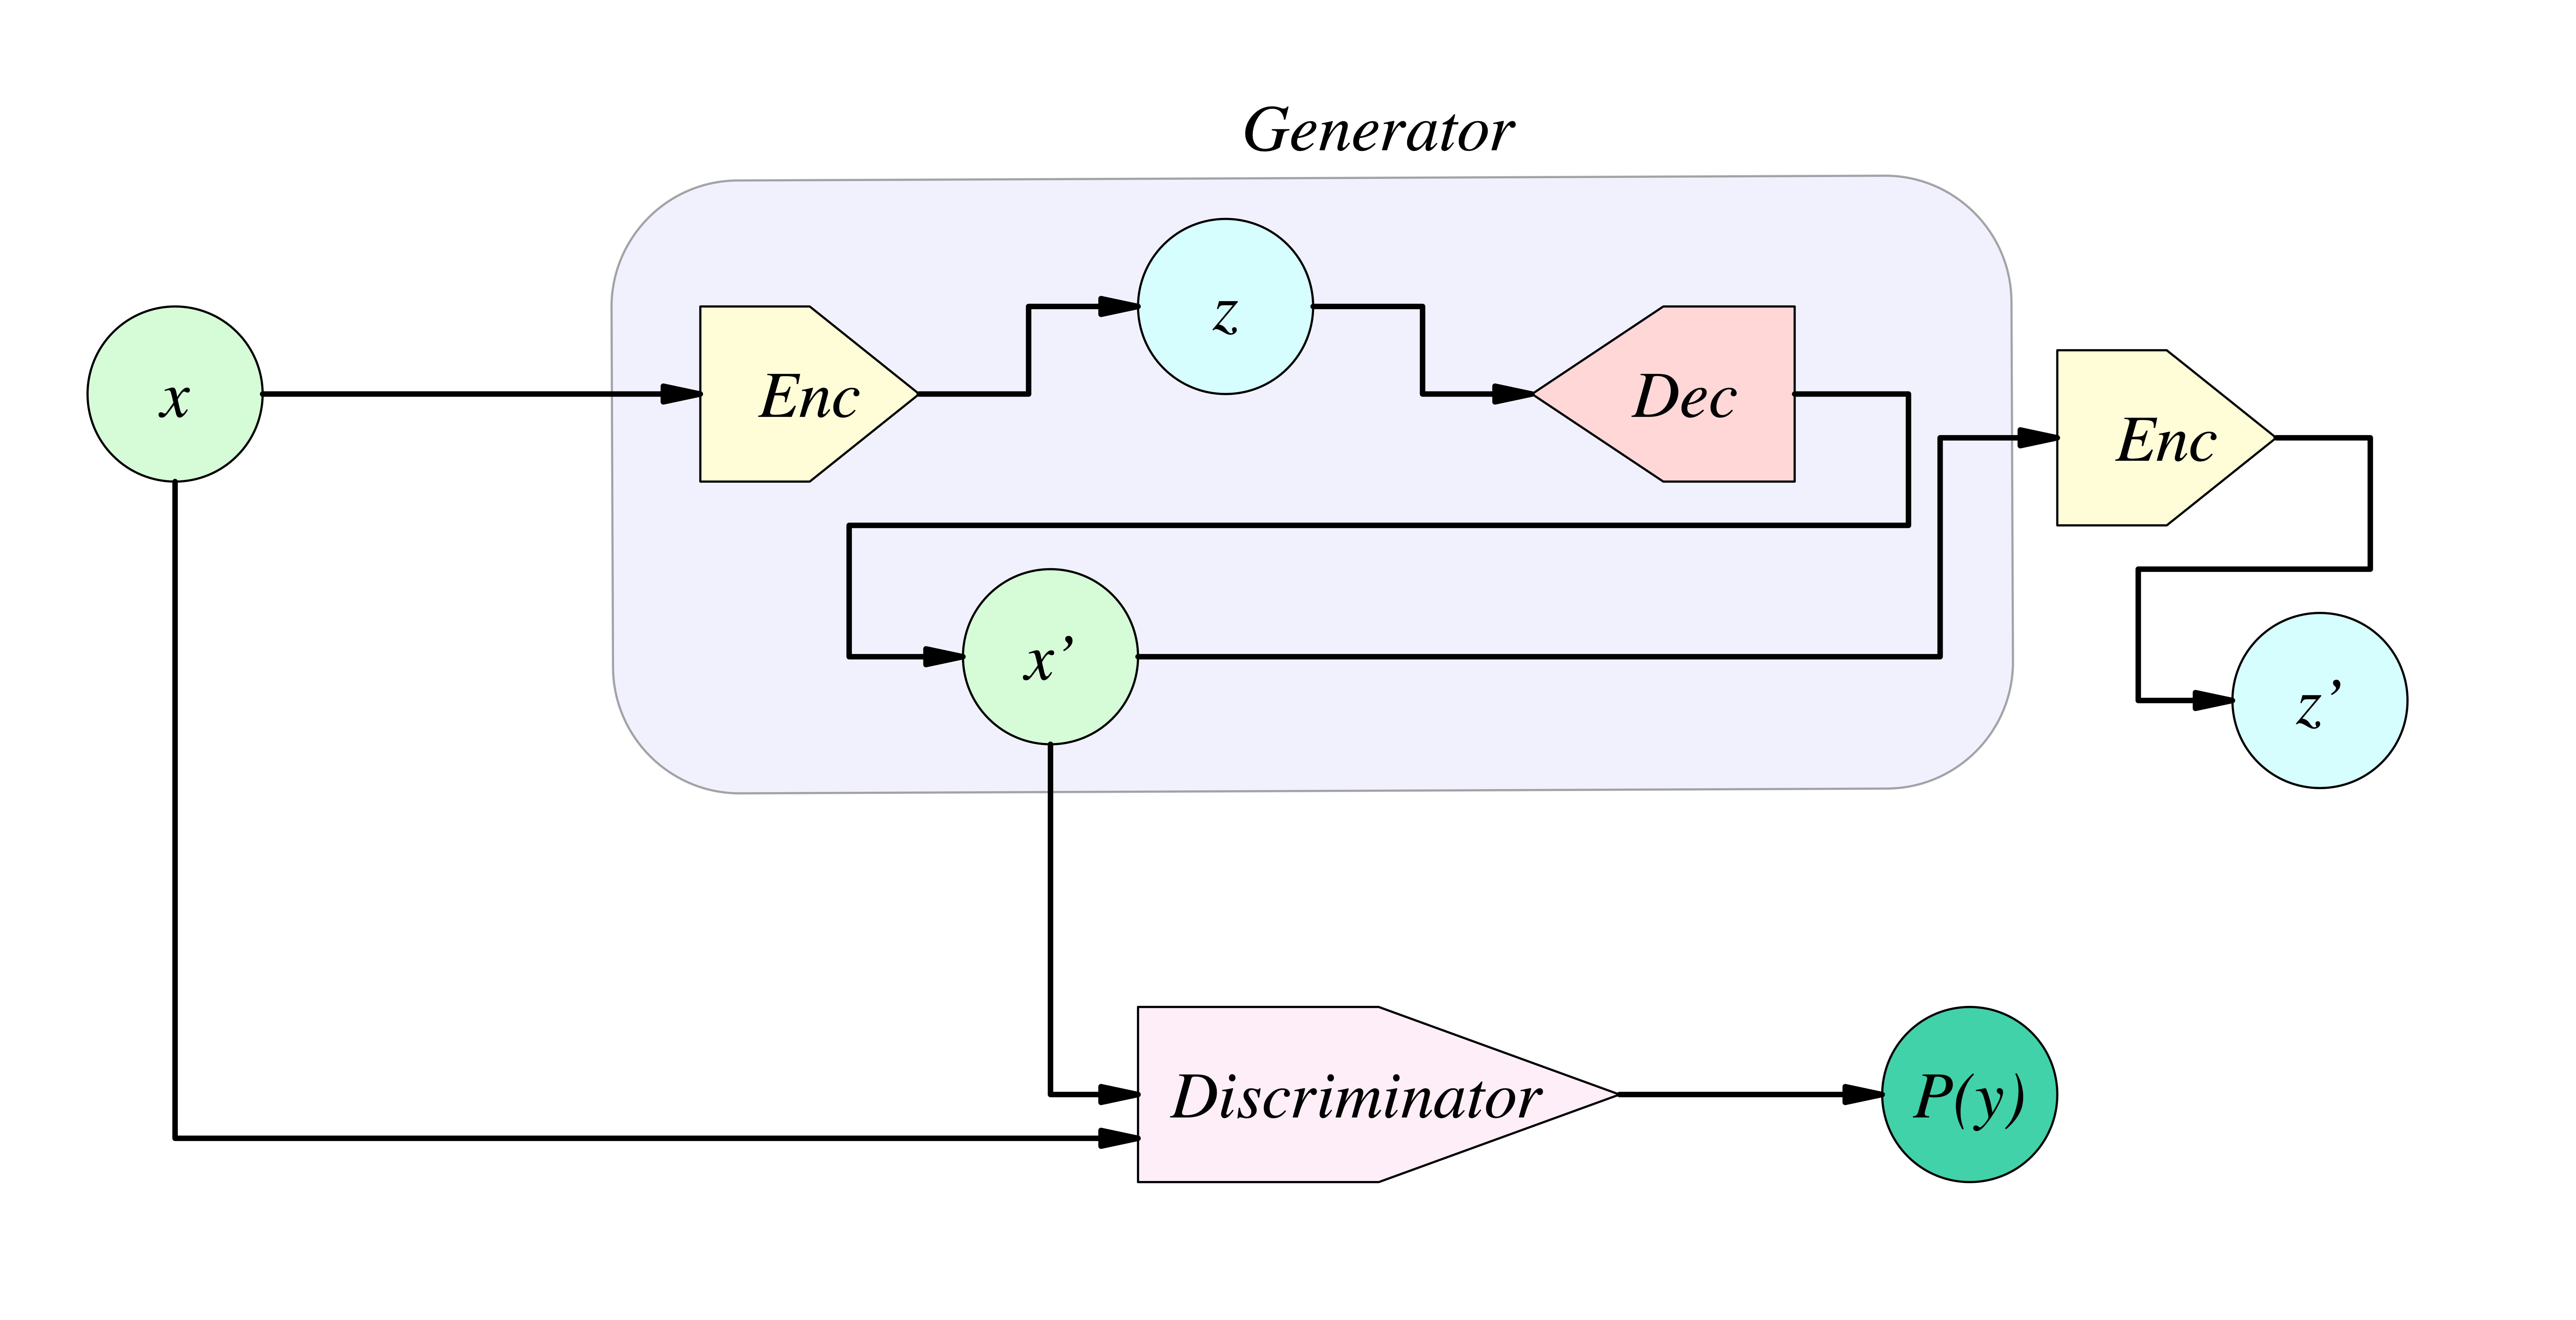
\includegraphics[width=.9\textwidth]{ganomaly}
    \caption{GANomaly architecture overview}
    \label{fig:ganomaly_model}
\end{figure}

 With the use of autoencoder network, framework obtains a superior reconstruction ability
compared to the previous models. But in doing so, its generative sub-network decoder is not a true
generative component from the perspective of the generative adversarial networks. Decoding capacity of the 
generator network of the GANomaly solely depends on the latent representations obtained from the generator's encoder
network. But in GAN, generator's decoding capabilities are more robust because it learns to generate samples from the 
distribution of the training data by training with an unsupervised fashion.

 With the change of the model architecture its training objective also changes. GANomaly model uses adversarial
training scheme but its generator network loss is the combination of 3 separate loss functions. These
are:
\begin{itemize}
   \item Adversarial Loss
   \item Contextual Loss
   \item Encoder Loss 
\end{itemize} 

\textbf{Adversarial loss} represents the loss function component for the adversarial training of the
framework. Instead of maximizing the probability of discriminator's attaining generated image as
real, it has a loss function derived from the \cite{fm} that uses feature matching. Main purpose
of this type of loss function is to reduce the instability in the GAN training. Adversarial loss
depicted in Equation \ref{eqn:ganomaly_adv} is the $\mathcal{L}_{2}$ distance of the feature
representation of the original and the generated image, respectively \cite{Akay2018GANomalySA}.
Feature layer is extracted from the activation layer before the output of the discriminator.  
\begin{equation}
    \label{eqn:ganomaly_adv}
    \mathcal{L}_{a d v}=\mathbb{E}_{x \sim p_{\mathbf{x}}}\left\|f(x)-\mathbb{E}_{x \sim p_{\mathbf{x}}} f\left(G(x) \|_{2}\right.\right. 
\end{equation}

Only adversarial loss does not help to optimize the generator towards reconstructing images similar
to the input data. To this end, \textbf{contextual loss} is also added to the generator loss function.
According to \cite{Isola2017ImagetoImageTW}, using $\mathcal{L}_1$ instead of $\mathcal{L}_2$
decreases the blurriness in the generated images, so the following contextual loss that measures the
distance between original image and the generated one is added to the to the total generator loss.
\begin{equation}
    \mathcal{L}_{c o n}=\mathbb{E}_{x \sim p_{\mathbf{X}}}\|x-G(x)\|_{1} 
\end{equation}

Additional \textbf{encoder loss} is also added to the generator to improve the encoding of the latent
representation of the reconstruction. This loss function aims to minimize the distance between the
encoded latent representation of the input image and the reconstruction. Loss function is
depicted below.
\begin{equation}
    \mathcal{L}_{e n c}=\mathbb{E}_{x \sim p_{\mathbf{X}}}\left\|G_{E}(x)-E(G(x))\right\|_{2} 
\end{equation}

Overall, the objective loss function of the generator is defined in Equation
\ref{eqn:ganomaly_oall} where the weight parameters $w_{adv}, w_{con} \text { and } w_{enc}$
are used to change the impact of individual losses.
\begin{equation}
    \label{eqn:ganomaly_oall}
    \mathcal{L}=w_{a d v} \mathcal{L}_{a d v}+w_{c o n} \mathcal{L}_{c o n}+w_{e n c} \mathcal{L}_{e n c} 
\end{equation}

GANomaly framework uses encoder loss function also as an anomaly score measure. Its execution is same 
as BiGAN and ALAD. 
\begin{equation}
\label{eqn:ganomaly_as}
    \mathcal{A}(\hat{x})=\left\|G_{E}(\hat{x})-E(G(\hat{x}))\right\|_{1}  
\end{equation}

Skip-GANomaly framework\cite{Akay2019SkipGANomalySC} is the continuation of the GANomaly architecture with changes mainly to the
generator network. As can be seen from Figure \ref{fig:sganomaly_model}, encoder and decoder
networks inside the generator framework is connected using skip connections. 
\begin{figure}[h!]
	\centering
	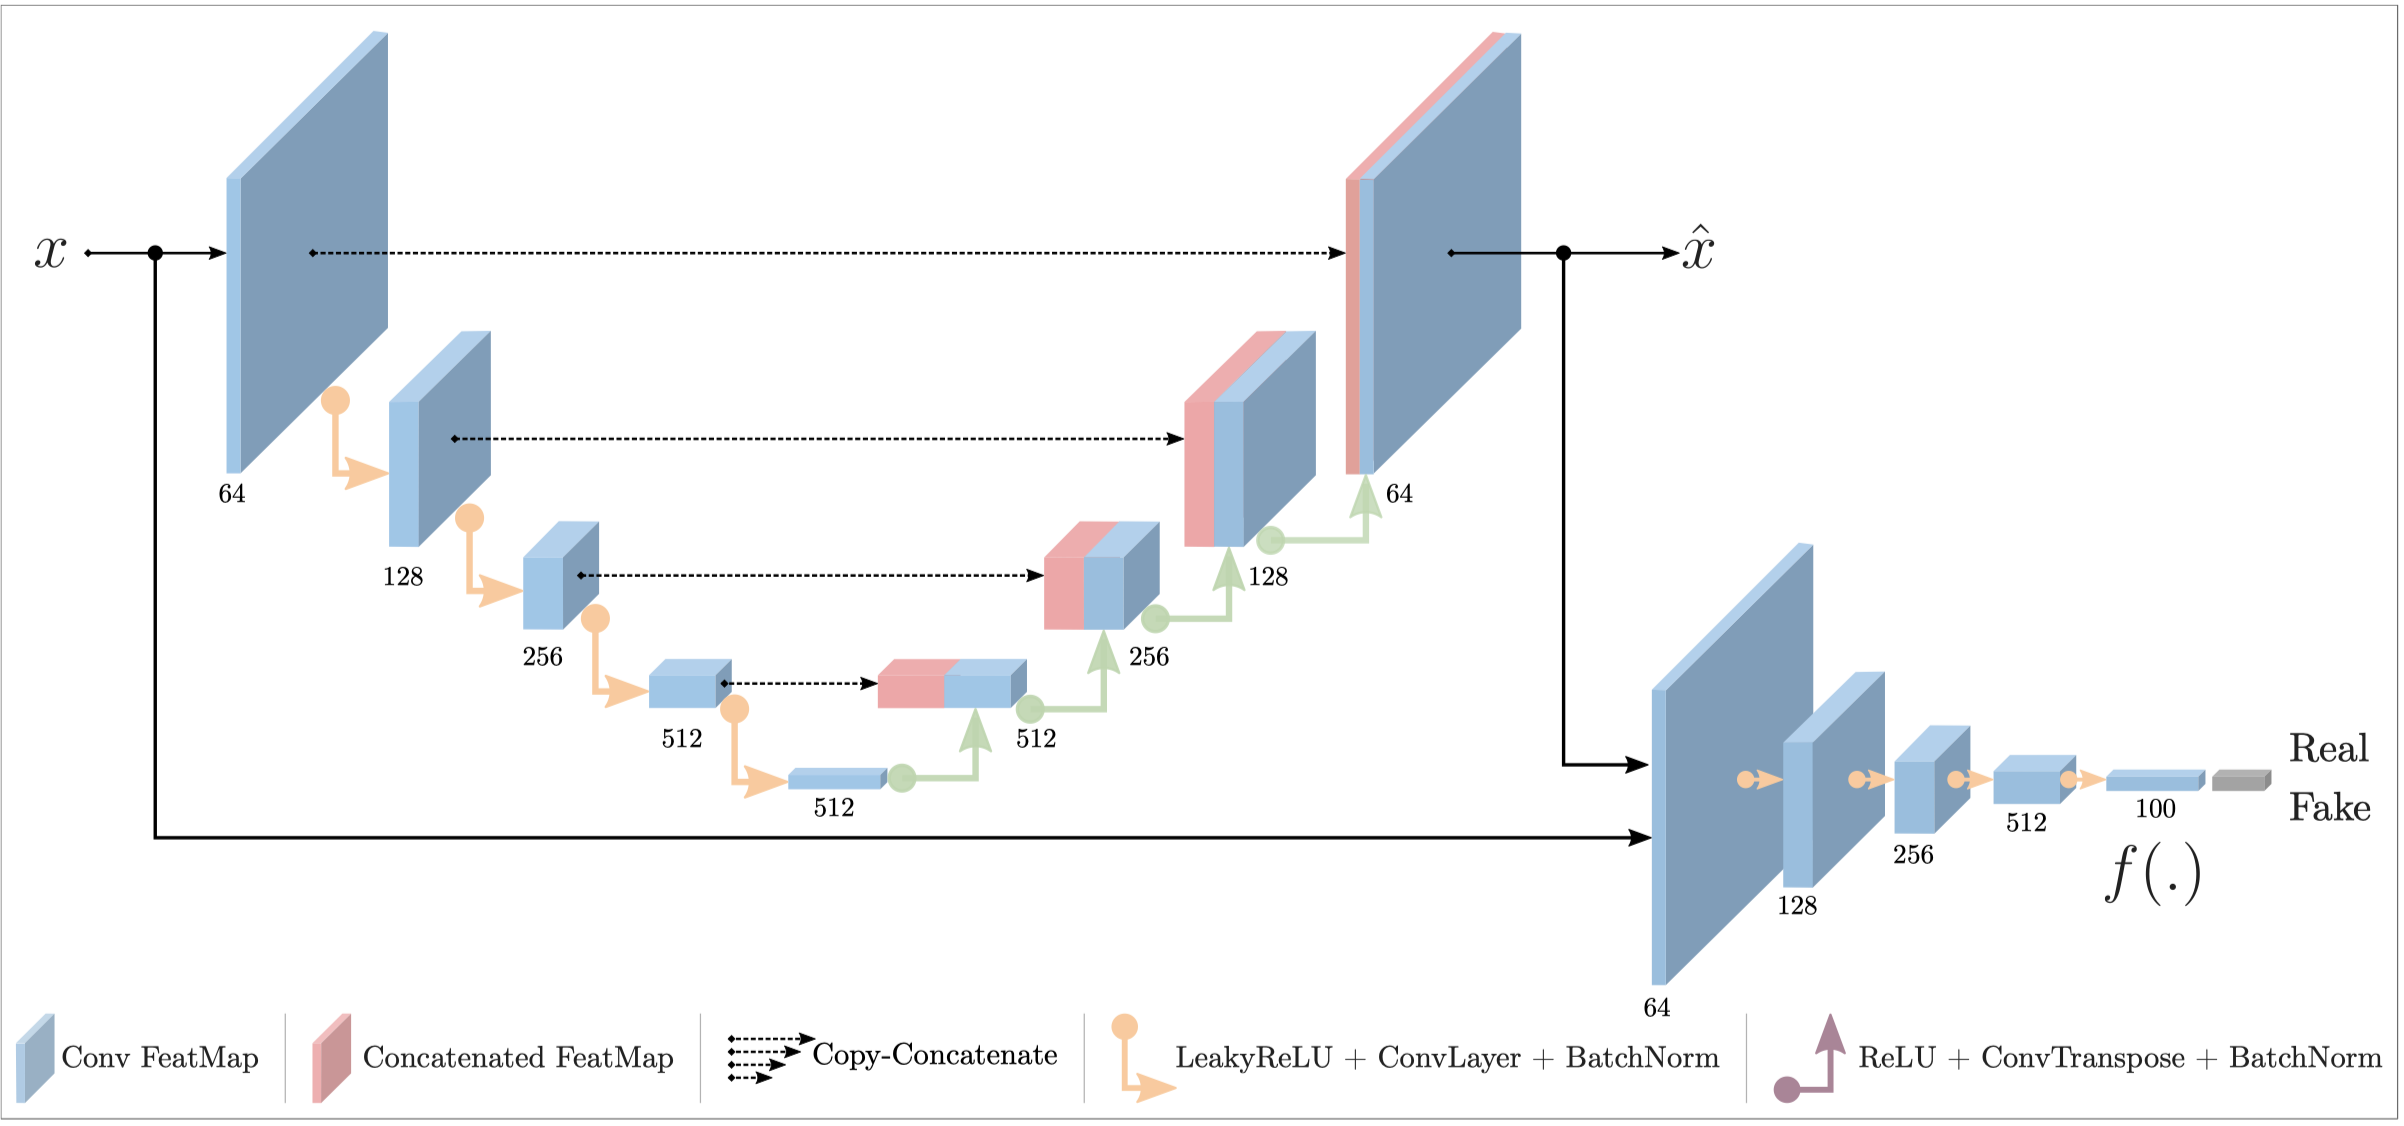
\includegraphics[width=.9\textwidth]{skip_ganomaly}
    \caption{Skip GANomaly architecture overview \cite{Akay2019SkipGANomalySC}}
    \label{fig:sganomaly_model}
\end{figure}

At each layer of the encoder, convolutional feature map is concatenated to the corresponding decoder
layer. Addition of skip connections provides a better reconstruction capability to the generator
than GANomaly framework \cite{Akay2018GANomalySA}. Training objective of the generator is the same as 
GANomaly model's with the exception of encoder loss. Because of the exclusion of the secondary 
encoder network, the encoder loss is obtained using the feature layer of the discriminator. 
\begin{equation}
    \mathcal{L}_{enc}=\underset{x \sim p_{x}}{\mathbb{E}}|f(x)-f(\hat{x})|_{2}  
\end{equation}

To find anomalies during the inference stage, Skip-GANomaly framework combines the encoder loss with
the use of contextual loss. 
\begin{equation}
	\label{eqn:sganomaly_as}
    \mathcal{A}(\dot{x})=\lambda R(\dot{x})+(1-\lambda) L(\dot{x})  
\end{equation}

$R(\dot{x})$ represents the contextual loss with the reconstruction term and $L(\dot{x})$ represents
the encoder loss with the latent representation term. Term $\lambda$ is used to adjust the impact of
the loss functions to the overall anomaly score.

Both GANomaly and Skip-GANomaly uses autoencoder network in their generator networks
and therefore have superior reconstruction capabilities compared to the previous 3 framework.
Primal problem with their architecture is that they don't adapt the true distribution of the input
data. They learn the underlying latent representation well to reconstruct the input and detect
anomalies. However their generator network represents the scenario where generator has learned the
input data distribution fairly well. In order to improve the results of a GAN based anomaly
detection framework, insights gained from these 2 networks are significantly important. Their
contribution to the improved framework and their performance analysis regards to other models will
be explored in Chapters \ref{chap:arim} and \ref{chap:expres} respectively. 

} %%%%%%%%% CONTROL POINT
%%%%%%%%%%%%%%%%%%%%%%%%%%
\endgroup
